\chapter{Apêndices}

\section{Diagrama da Classe RF24}
  \begin{figure}[!htb]
    \centering
    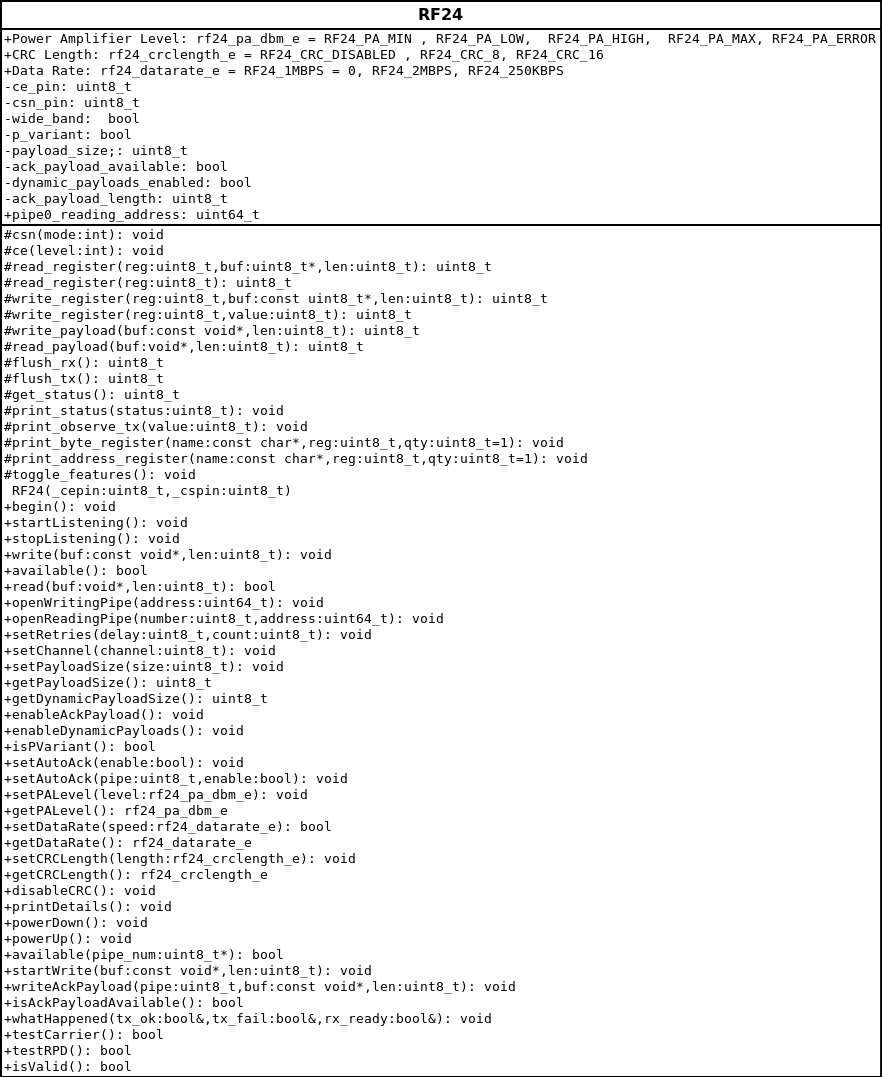
\includegraphics[width=\linewidth]{../../Imagens/RF24_class.png}
    \caption{Diagrama da Classe RF24} %% TODO certificar se realmente é uma WBS!!!
    \label{RF24_ClassDiag}
  \end{figure}

\section{Estrutura Analítica do Projeto}
  \begin{figure}[!htb] %% TODO certificar se realmente é uma WBS!!!
    \centering
    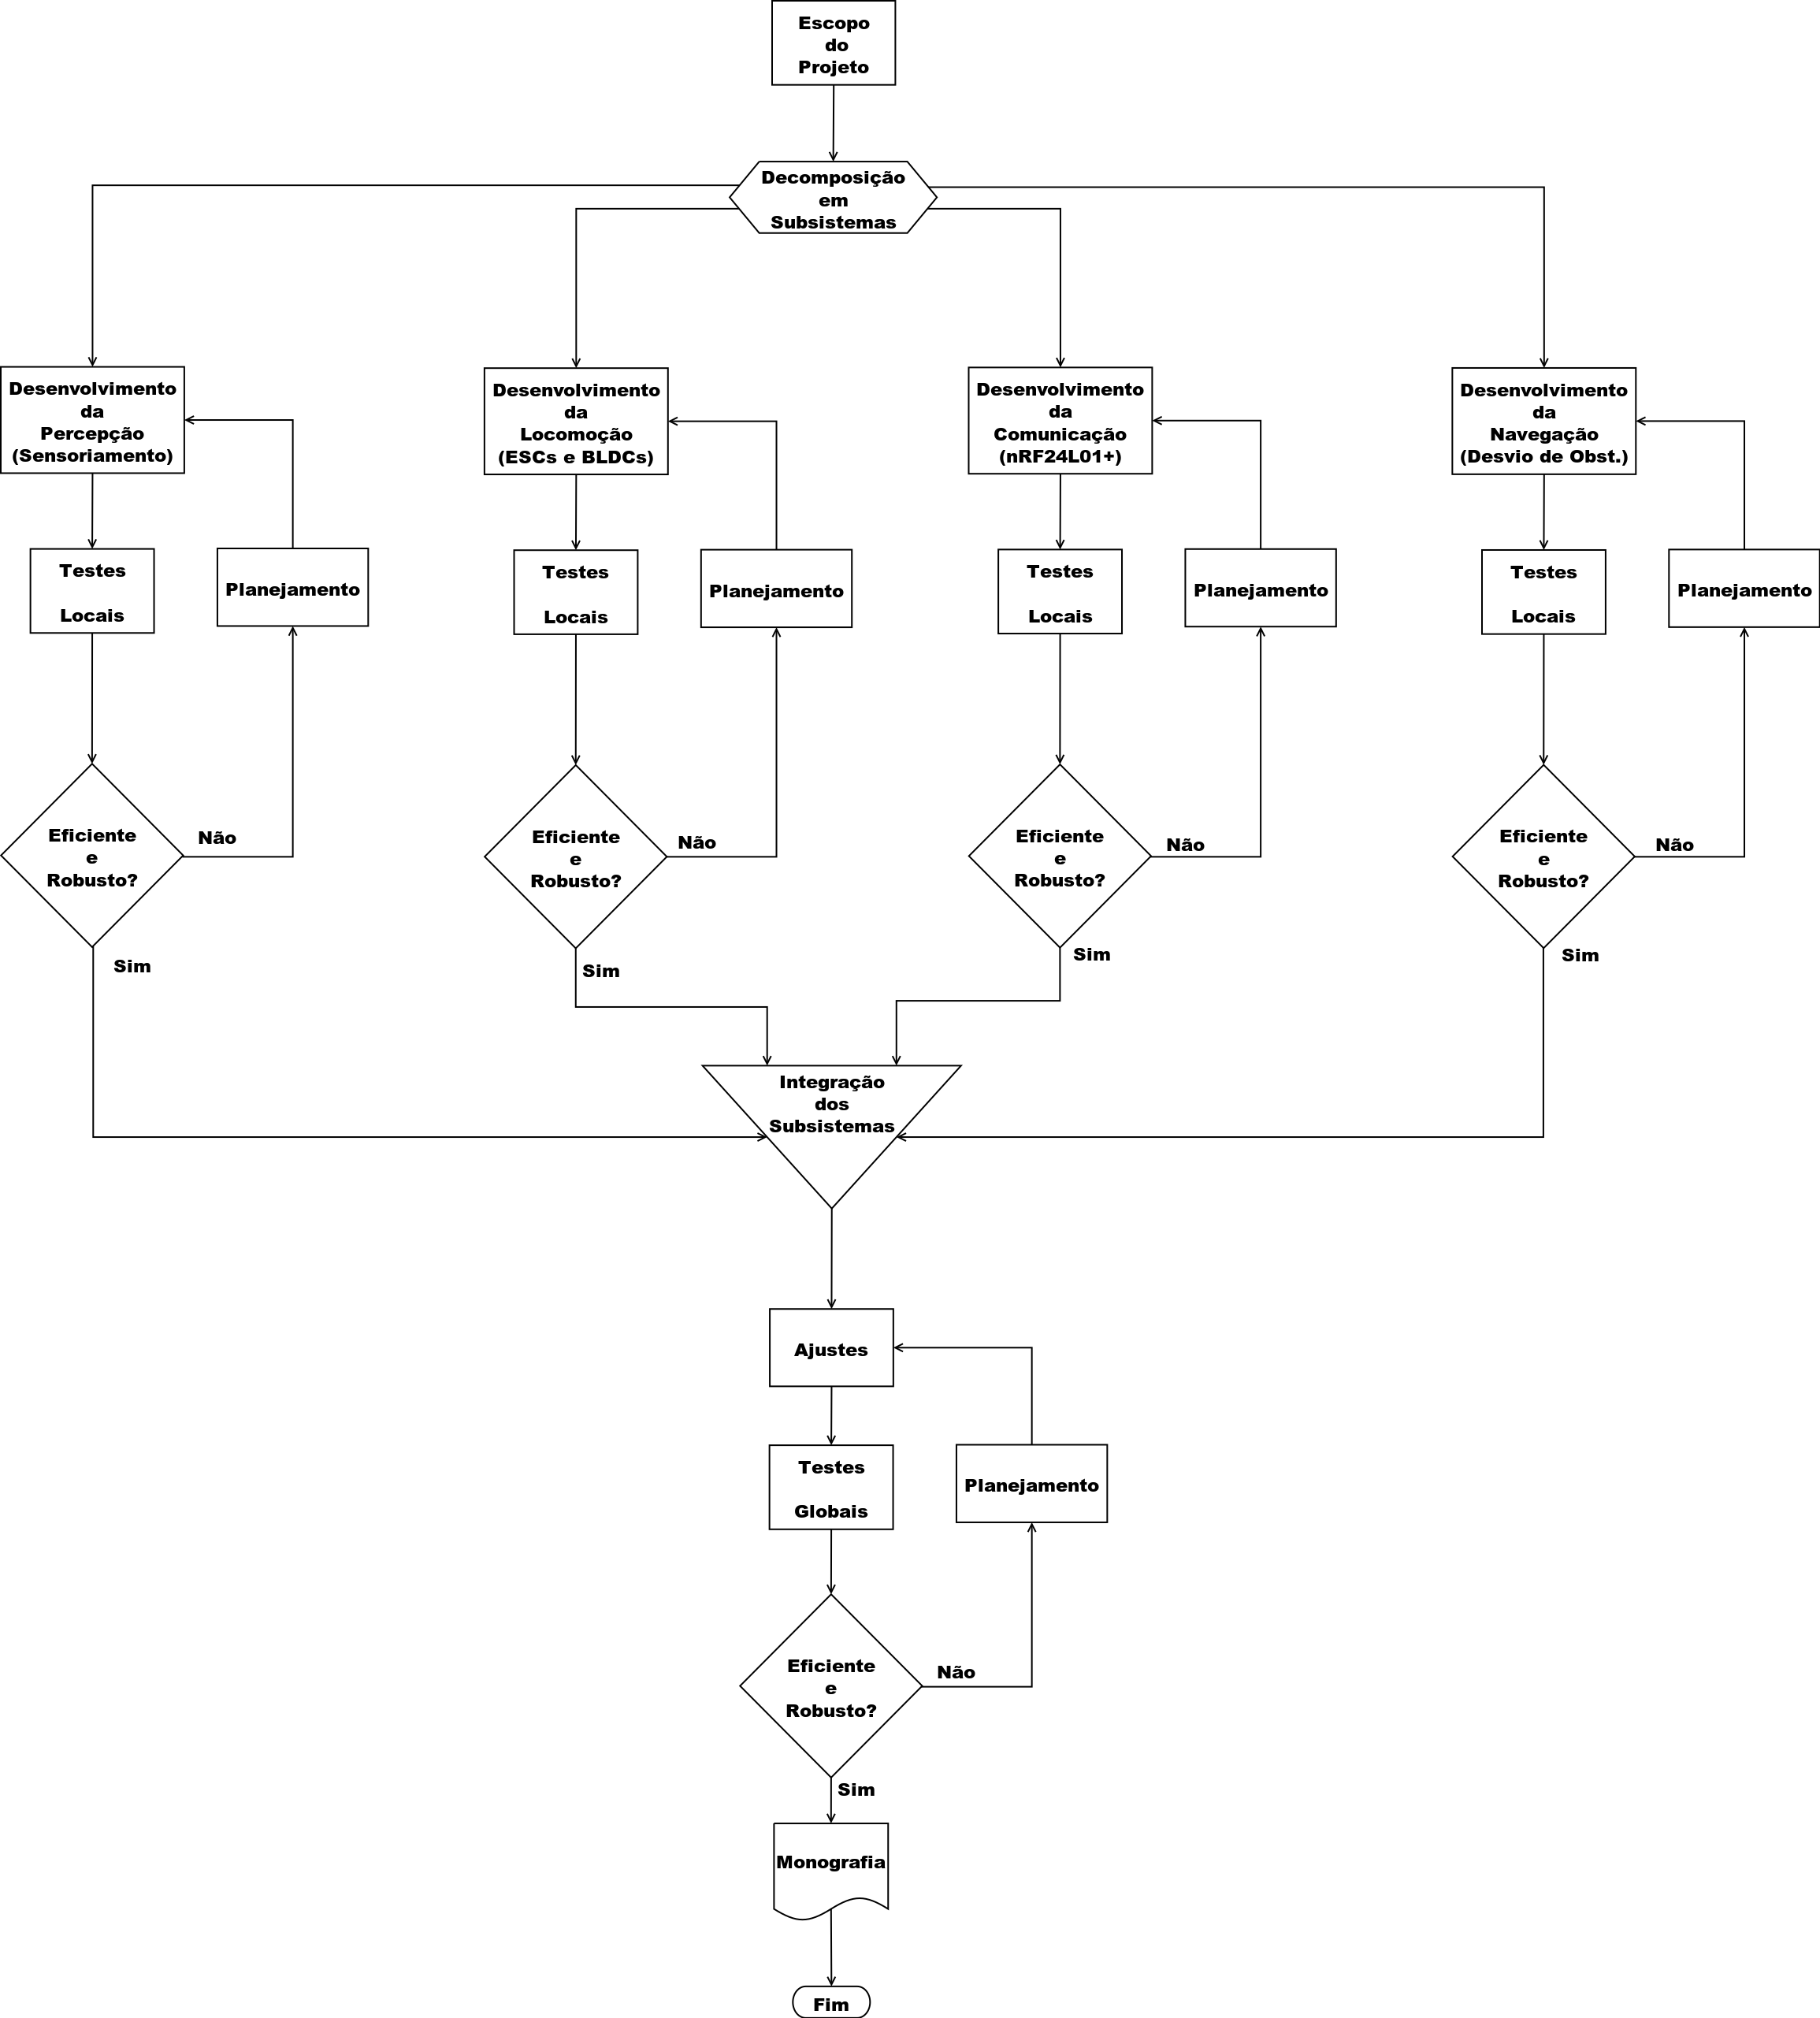
\includegraphics[width=\linewidth]{../../Imagens/WBS.png}
    \caption{Estrutura Analítica do Projeto} %% TODO certificar se realmente é uma WBS!!!
    \label{WBS}
  \end{figure}
  
\section{Esquemático do Robô}
  \begin{figure}[!htb]
    \centering
    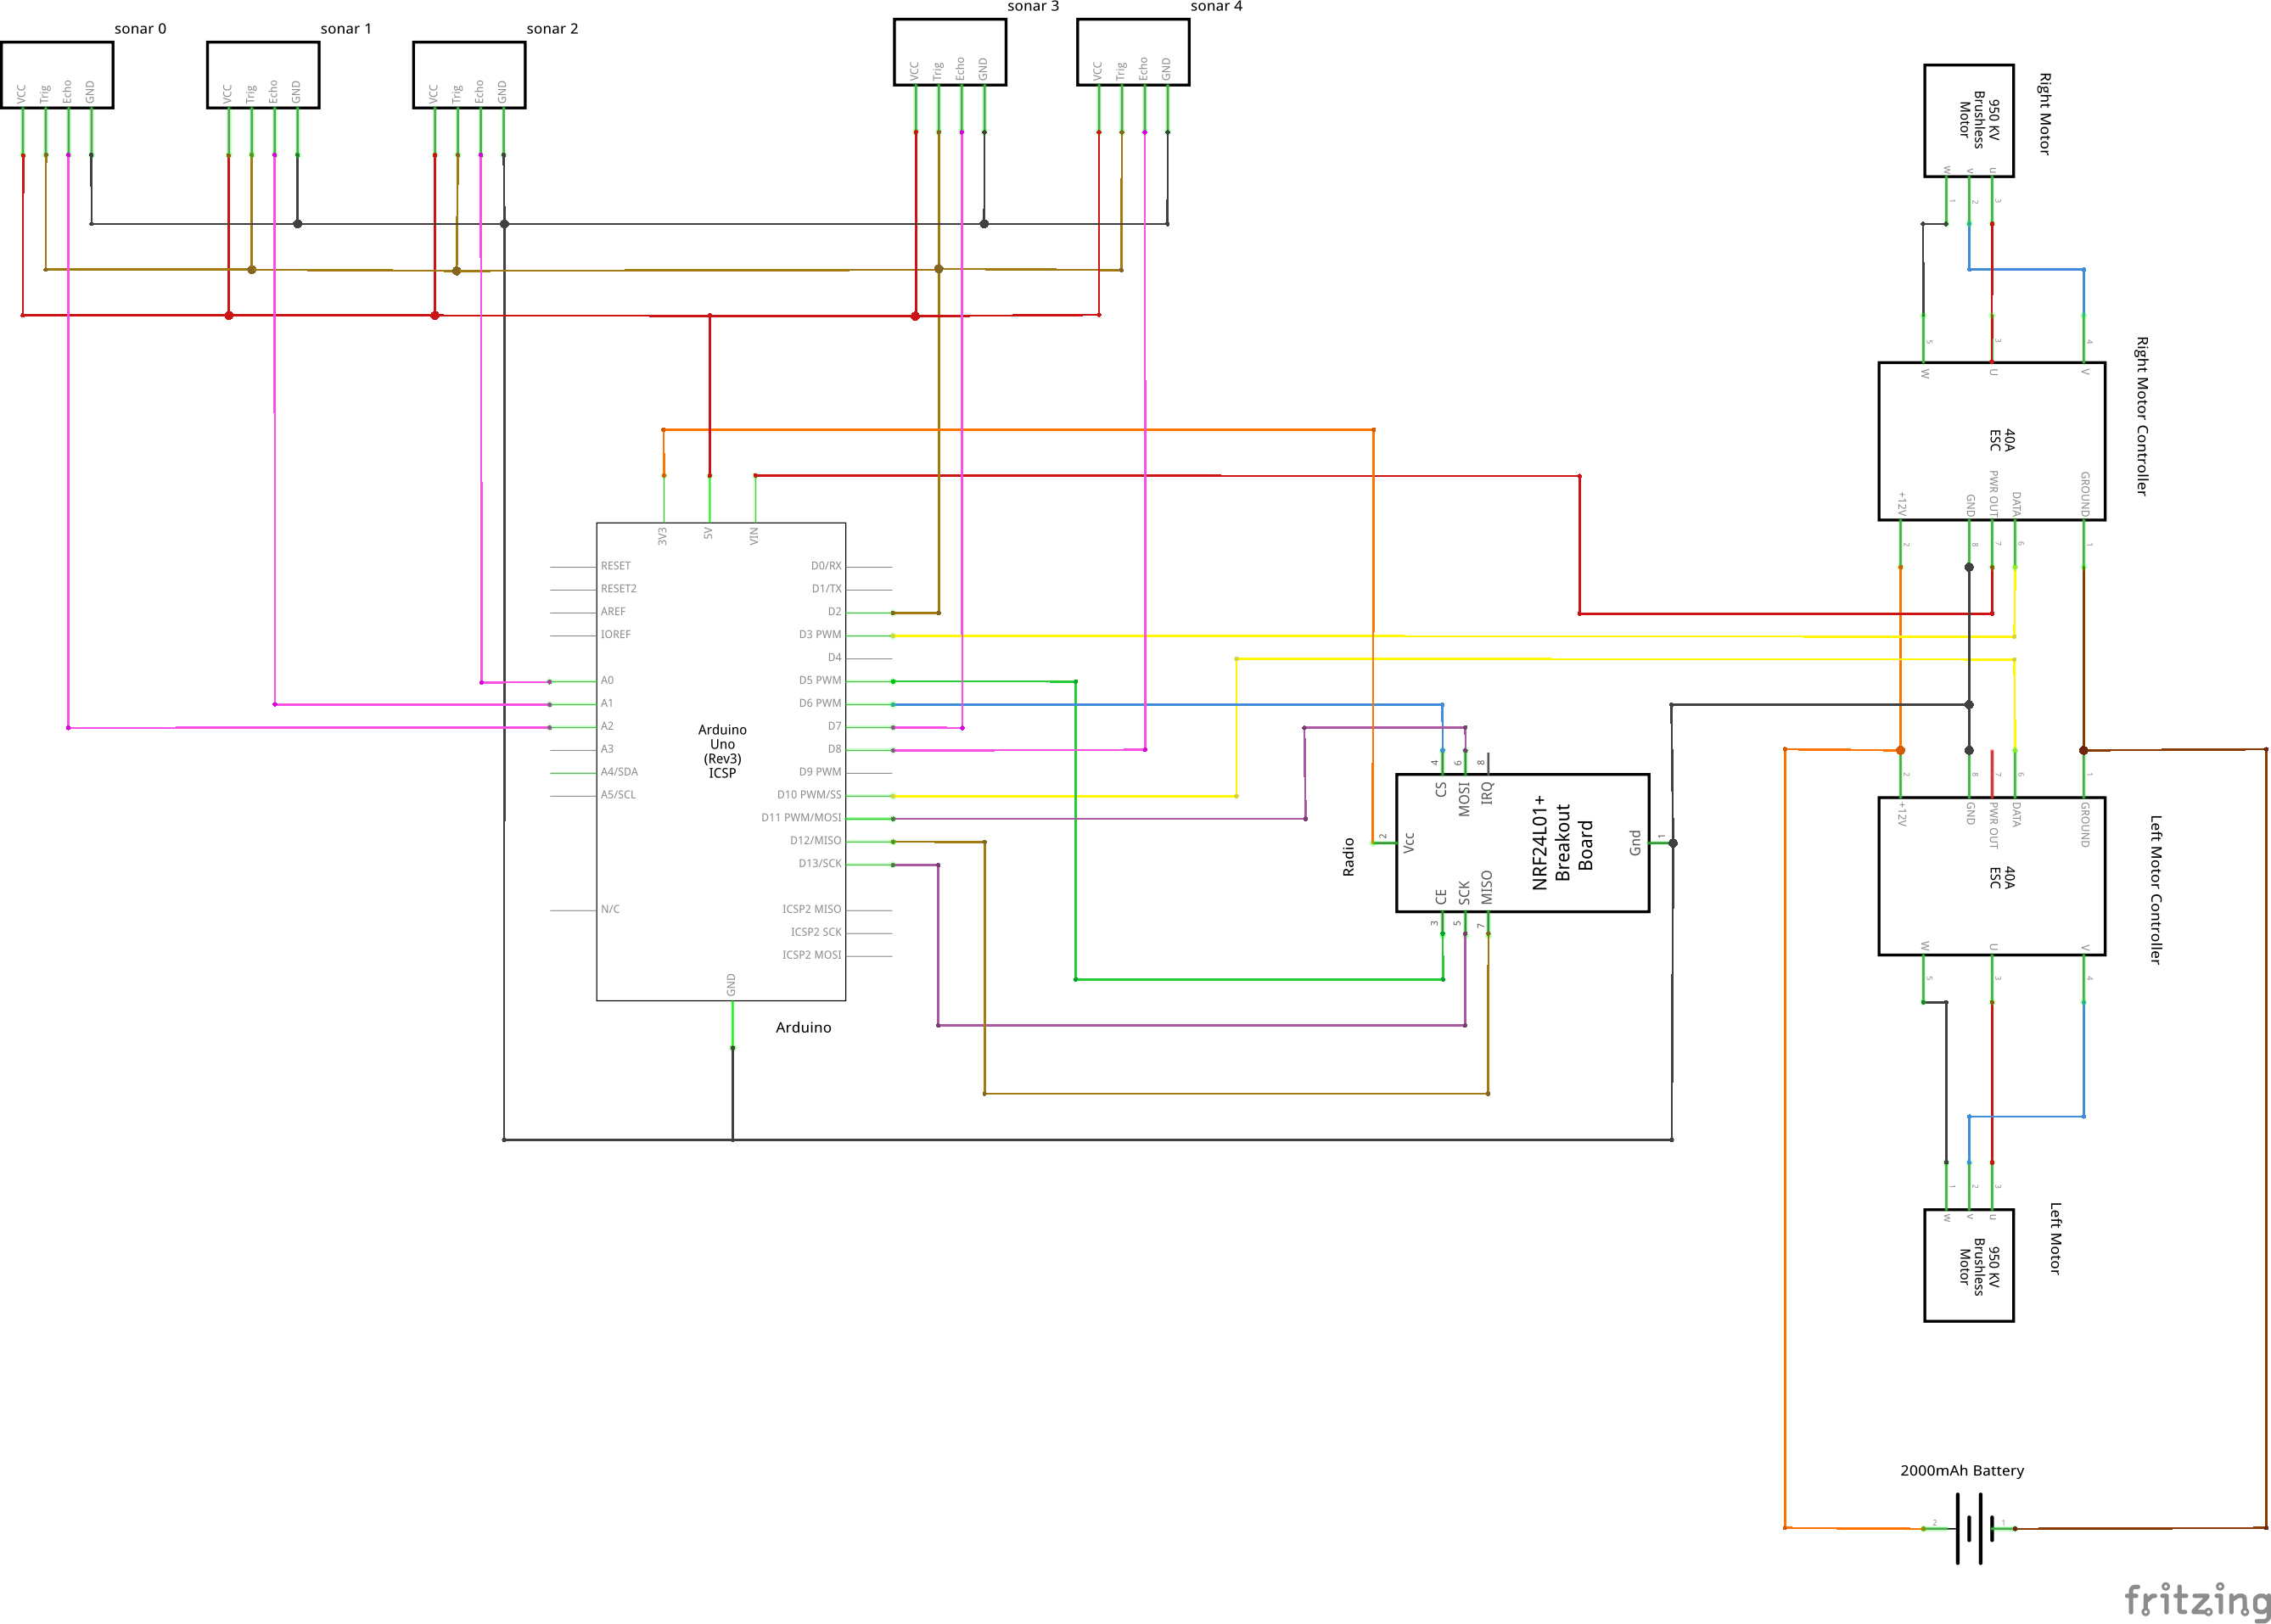
\includegraphics[width=\linewidth]{../../Imagens/robot_schem.png}
    \caption{Diagrama Elétrico} %% TODO: é um bom nome??
    \label{fritzing}
  \end{figure}
  
% TODO desatualizada!!!!
\section{Tabela Verdade}
% TODO desatualizada!!!!
\begin{table}[!htb]
\centering
\caption{}
\label{IA}
\begin{tabular}{|ccccc|c|}
\hline
{\color[HTML]{00009B} \textbf{$USS_0$}} & {\color[HTML]{00009B} \textbf{$USS_1$}} & {\color[HTML]{00009B} \textbf{$USS_2$}} & 
{\color[HTML]{00009B} \textbf{$USS_3$}} & {\color[HTML]{00009B} \textbf{$USS_4$}} & {\color[HTML]{FE0000} \textbf{Ação}} \\ 
\hline
{\color[HTML]{00009B} 0}                                     & {\color[HTML]{00009B} 0}                                    & {\color[HTML]{00009B} 0} 
 
                                  & {\color[HTML]{00009B} 0}                                    & {\color[HTML]{00009B} 1}                            
 
       & {\color[HTML]{FE0000} $E_L$}                                     \\ \hline
{\color[HTML]{00009B} 0}                                     & {\color[HTML]{00009B} 0}                                    & {\color[HTML]{00009B} 0} 
 
                                  & {\color[HTML]{00009B} 1}                                    & {\color[HTML]{00009B} 0}                            
 
       & {\color[HTML]{FE0000} $E_M$}                                     \\ \hline
{\color[HTML]{00009B} 0}                                     & {\color[HTML]{00009B} 0}                                    & {\color[HTML]{00009B} 0} 
 
                                  & {\color[HTML]{00009B} 1}                                    & {\color[HTML]{00009B} 1}                            
 
       & {\color[HTML]{FE0000} $E_M$}                                     \\ \hline
{\color[HTML]{00009B} 0}                                     & {\color[HTML]{00009B} 0}                                    & {\color[HTML]{00009B} 1} 
 
                                  & {\color[HTML]{00009B} 0}                                    & {\color[HTML]{00009B} 0}                            
 
       & {\color[HTML]{FE0000} $E_F$}                                     \\ \hline
{\color[HTML]{00009B} 0}                                     & {\color[HTML]{00009B} 0}                                    & {\color[HTML]{00009B} 1} 
 
                                  & {\color[HTML]{00009B} 0}                                    & {\color[HTML]{00009B} 1}                            
 
       & {\color[HTML]{FE0000} $E_F$}                                     \\ \hline
{\color[HTML]{00009B} 0}                                   & {\color[HTML]{00009B} 0}                                    & {\color[HTML]{00009B} 1}   
 
                                & {\color[HTML]{00009B} 1}                                    & {\color[HTML]{00009B} 0}                              
 
     & {\color[HTML]{FE0000} $E_F$}                                     \\ \hline
{\color[HTML]{00009B} 0}                                    & {\color[HTML]{00009B} 0}                                  & {\color[HTML]{00009B} 1}    
 
                               & {\color[HTML]{00009B} 1}                                    & {\color[HTML]{00009B} 1}                               
 
    & {\color[HTML]{FE0000} $E_F$}                                     \\ \hline
{\color[HTML]{00009B} 0}                                     & {\color[HTML]{00009B} 1}                                    & {\color[HTML]{00009B} 0} 
 
                                & {\color[HTML]{00009B} 0}                                    & {\color[HTML]{00009B} 0}                              
 
     & {\color[HTML]{FE0000} $D_M$}                                     \\ \hline
{\color[HTML]{00009B} 0}                                    & {\color[HTML]{00009B} 1}                                    & {\color[HTML]{00009B} 0}  
 
                                 & {\color[HTML]{00009B} 0}                                 & {\color[HTML]{00009B} 1}                                
 
   & {\color[HTML]{FE0000} $D_M$}                                     \\ \hline
{\color[HTML]{00009B} 0}                                    & {\color[HTML]{00009B} 1}                                    & {\color[HTML]{00009B} 0}  
 
                                 & {\color[HTML]{00009B} 1}                                    & {\color[HTML]{00009B} 0}                             
 
      & {\color[HTML]{FE0000} $E_F$}                                     \\ \hline
{\color[HTML]{00009B} 0}                                    & {\color[HTML]{00009B} 1}                                    & {\color[HTML]{00009B} 0}  
 
                                 & {\color[HTML]{00009B} 1}                                    & {\color[HTML]{00009B} 1}                             
 
      & {\color[HTML]{FE0000} $E_M$}                                  \\ \hline
{\color[HTML]{00009B} 0}                                     & {\color[HTML]{00009B} 1}                                    & {\color[HTML]{00009B} 1} 
 
                                  & {\color[HTML]{00009B} 0}                                    & {\color[HTML]{00009B} 0}                            
 
       & {\color[HTML]{FE0000} $D_F$}                                     \\ \hline
{\color[HTML]{00009B} 0}                                     & {\color[HTML]{00009B} 1}                                    & {\color[HTML]{00009B} 1} 
 
                                  & {\color[HTML]{00009B} 0}                                    & {\color[HTML]{00009B} 1}                            
 
       & {\color[HTML]{FE0000} $E_F$}                                     \\ \hline
{\color[HTML]{00009B} 0}                                     & {\color[HTML]{00009B} 1}                                    & {\color[HTML]{00009B} 1} 
 
                                  & {\color[HTML]{00009B} 1}                                    & {\color[HTML]{00009B} 0}                            
 
       & {\color[HTML]{FE0000} $E_F$}                                     \\ \hline
{\color[HTML]{00009B} 0}                                     & {\color[HTML]{00009B} 1}                                    & {\color[HTML]{00009B} 1} 
 
                                  & {\color[HTML]{00009B} 1}                                    & {\color[HTML]{00009B} 1}                            
 
       & {\color[HTML]{FE0000} $E_F$}                                     \\ \hline
{\color[HTML]{00009B} 1}                                     & {\color[HTML]{00009B} 0}                                    & {\color[HTML]{00009B} 0} 
 
                                  & {\color[HTML]{00009B} 0}                                    & {\color[HTML]{00009B} 0}                            
 
       & {\color[HTML]{FE0000} $D_L$}                                     \\ \hline
{\color[HTML]{00009B} 1}                                     & {\color[HTML]{00009B} 0}                                    & {\color[HTML]{00009B} 0} 
 
                                  & {\color[HTML]{00009B} 0}                                    & {\color[HTML]{00009B} 1}                            
 
       & {\color[HTML]{FE0000} Frente}                                     \\ \hline
{\color[HTML]{00009B} 1}                                     & {\color[HTML]{00009B} 0}                                    & {\color[HTML]{00009B} 0} 
 
                                  & {\color[HTML]{00009B} 1}                                    & {\color[HTML]{00009B} 0}                            
 
       & {\color[HTML]{FE0000} $E_M$}                                     \\ \hline
{\color[HTML]{00009B} 1}                                     & {\color[HTML]{00009B} 0}                                    & {\color[HTML]{00009B} 0} 
 
                                  & {\color[HTML]{00009B} 1}                                    & {\color[HTML]{00009B} 1}                            
 
       & {\color[HTML]{FE0000} $E_M$}                                     \\ \hline
{\color[HTML]{00009B} 1}                                     & {\color[HTML]{00009B} 0}                                    & {\color[HTML]{00009B} 1} 
 
                                  & {\color[HTML]{00009B} 0}                                    & {\color[HTML]{00009B} 0}                            
 
       & {\color[HTML]{FE0000} $D_F$}                                     \\ \hline
{\color[HTML]{00009B} 1}                                     & {\color[HTML]{00009B} 0}                                    & {\color[HTML]{00009B} 1} 
 
                                  & {\color[HTML]{00009B} 0}                                    & {\color[HTML]{00009B} 1}                            
 
       & {\color[HTML]{FE0000} $E_F$}                                     \\ \hline
{\color[HTML]{00009B} 1}                                     & {\color[HTML]{00009B} 0}                                    & {\color[HTML]{00009B} 1} 
 
                                  & {\color[HTML]{00009B} 1}                                    & {\color[HTML]{00009B} 0}                            
 
       & {\color[HTML]{FE0000} $E_F$}                                     \\ \hline
{\color[HTML]{00009B} 1}                                     & {\color[HTML]{00009B} 0}                                    & {\color[HTML]{00009B} 1} 
 
                                  & {\color[HTML]{00009B} 1}                                    & {\color[HTML]{00009B} 1}                            
 
       & {\color[HTML]{FE0000} $E_F$}                                     \\ \hline
{\color[HTML]{00009B} 1}                                     & {\color[HTML]{00009B} 1}                                    & {\color[HTML]{00009B} 0} 
 
                                  & {\color[HTML]{00009B} 0}                                    & {\color[HTML]{00009B} 0}                            
 
       & {\color[HTML]{FE0000} $D_M$}                                     \\ \hline
{\color[HTML]{00009B} 1}                                     & {\color[HTML]{00009B} 1}                                    & {\color[HTML]{00009B} 0} 
 
                                  & {\color[HTML]{00009B} 0}                                    & {\color[HTML]{00009B} 1}                            
 
       & {\color[HTML]{FE0000} $D_M$}                                     \\ \hline
{\color[HTML]{00009B} 1}                                     & {\color[HTML]{00009B} 1}                                    & {\color[HTML]{00009B} 0} 
 
                                  & {\color[HTML]{00009B} 1}                                    & {\color[HTML]{00009B} 0}                            
 
       & {\color[HTML]{FE0000} $D_M$}                                     \\ \hline
{\color[HTML]{00009B} 1}                                     & {\color[HTML]{00009B} 1}                                    & {\color[HTML]{00009B} 0} 
 
                                  & {\color[HTML]{00009B} 1}                                    & {\color[HTML]{00009B} 1}                            
 
       & {\color[HTML]{FE0000} Frente}                                     \\ \hline
{\color[HTML]{00009B} 1}                                     & {\color[HTML]{00009B} 1}                                    & {\color[HTML]{00009B} 1} 
 
                                  & {\color[HTML]{00009B} 0}                                    & {\color[HTML]{00009B} 0}                            
 
       & {\color[HTML]{FE0000} $D_F$}                                     \\ \hline
{\color[HTML]{00009B} 1}                                     & {\color[HTML]{00009B} 1}                                    & {\color[HTML]{00009B} 1} 
 
                                  & {\color[HTML]{00009B} 0}                                    & {\color[HTML]{00009B} 1}                            
 
       & {\color[HTML]{FE0000} $D_F$}                                     \\ \hline
{\color[HTML]{00009B} 1}                                     & {\color[HTML]{00009B} 1}                                    & {\color[HTML]{00009B} 1} 
 
                                  & {\color[HTML]{00009B} 1}                                    & {\color[HTML]{00009B} 0}                            
 
       & {\color[HTML]{FE0000} $D_F$}                                     \\ \hline
{\color[HTML]{00009B} 1}                                     & {\color[HTML]{00009B} 1}                                    & {\color[HTML]{00009B} 1} 
 
                                  & {\color[HTML]{00009B} 1}                                    & {\color[HTML]{00009B} 1}                            
 
       & {\color[HTML]{FE0000} $E_F$}                                    \\ \hline

\end{tabular}
\end{table}



\section{Testes}

\subsection{Leituras Dinâmicas}
\begin{table}[]
\centering
\caption{My caption}
\label{my-label}
\begin{tabular}{|c|c|ccccc|}
\hline
\textbf{Teste}            & \textbf{Medida}                                                            & \textbf{Sensor 0}         & \textbf{Sensor 1}         & \textbf{Sensor 2}         & \textbf{Sensor 3}         & \textbf{Sensor 4}          \\ \hline
1                         & Média                                                                      & 26,58                     & 30,57                     & 30,55                     & 35,67                     & 37,51                      \\
2                         & Média                                                                      & 26,42                     & 30,60                     & 32,17                     & 35,61                     & 37,52                      \\
3                         & Média                                                                      & 26,39                     & 30,86                     & 32,31                     & 35,76                     & 37,73                      \\
4                         & Média                                                                      & 26,42                     & 30,29                     & 29,11                     & 35,65                     & 37,36                      \\
5                         & Média                                                                      & 26,72                     & 30,48                     & 31,11                     & 35,71                     & 37,65                      \\
6                         & Média                                                                      & 26,52                     & 30,35                     & 28,47                     & 35,50                     & 37,33                      \\ \hline
1                         & Média Limpa                                                                & 26,58                     & 30,57                     & 30,55                     & 35,67                     & 37,51                      \\
2                         & Média Limpa                                                                & 26,42                     & 30,60                     & 32,17                     & 35,61                     & 37,52                      \\
3                         & Média Limpa                                                                & 26,39                     & 30,86                     & 32,31                     & 35,76                     & 37,73                      \\
4                         & Média Limpa                                                                & 26,42                     & 30,29                     & 29,11                     & 35,65                     & 37,36                      \\
5                         & Média Limpa                                                                & 26,72                     & 30,48                     & 31,11                     & 35,71                     & 37,65                      \\
6                         & Média Limpa                                                                & 26,52                     & 30,35                     & 28,47                     & 35,50                     & 37,33                      \\ \hline
1                         & Desvio Padrão                                                              & 0,50                      & 0,50                      & 4,19                      & 0,55                      & 0,53                       \\
2                         & Desvio Padrão                                                              & 0,50                      & 0,49                      & 4,35                      & 0,59                      & 0,55                       \\
3                         & Desvio Padrão                                                              & 0,49                      & 0,35                      & 4,12                      & 0,54                      & 0,62                       \\
4                         & Desvio Padrão                                                              & 0,50                      & 0,46                      & 8,18                      & 0,48                      & 0,63                       \\
5                         & Desvio Padrão                                                              & 0,45                      & 0,50                      & 4,10                      & 0,50                      & 0,69                       \\
6                         & Desvio Padrão                                                              & 0,50                      & 0,48                      & 7,47                      & 0,50                      & 0,49                       \\ \hline
1                         & Desvio Padrão Limpo                                                        & 0,50                      & 0,50                      & 4,19                      & 0,55                      & 0,53                       \\
2                         & Desvio Padrão Limpo                                                        & 0,50                      & 0,49                      & 4,35                      & 0,59                      & 0,55                       \\
3                         & Desvio Padrão Limpo                                                        & 0,49                      & 0,35                      & 4,12                      & 0,54                      & 0,62                       \\
4                         & Desvio Padrão Limpo                                                        & 0,50                      & 0,46                      & 8,18                      & 0,48                      & 0,63                       \\
5                         & Desvio Padrão Limpo                                                        & 0,45                      & 0,50                      & 4,10                      & 0,50                      & 0,69                       \\
6                         & Desvio Padrão Limpo                                                        & 0,50                      & 0,48                      & 7,47                      & 0,50                      & 0,49                       \\ \hline
1                         & \textless (Média)/2                                                        & 0\%                    & 0\%                    & 2,67\%                    & 0\%                    & 0\%                     \\
2                         & \textless (Média)/2                                                        & 0\%                    & 0\%                    & 2,00\%                    & 0\%                    & 0\%                     \\
3                         & \textless (Média)/2                                                        & 0\%                    & 0\%                    & 2,00\%                    & 0\%                    & 0\%                     \\
4                         & \textless (Média)/2                                                        & 0\%                    & 0\%                    & 11,33\%                   & 0\%                    & 0\%                     \\
5                         & \textless (Média)/2                                                        & 0\%                    & 0\%                    & 2,00\%                    & 0\%                    & 0\%                     \\
6                         & \textless (Média)/2                                                        & 0\%                    & 0\%                    & 10,00\%                   & 0\%                    & 0\%                     \\ \hline
1                         & Destoantes                                                                 & 0\%                    & 0\%                    & 0\%                    & 0\%                    & 0\%                     \\
2                         & Destoantes                                                                 & 0\%                    & 0\%                    & 0\%                    & 0\%                    & 0\%                     \\
3                         & Destoantes                                                                 & 0\%                    & 0\%                    & 0\%                    & 0\%                    & 0\%                     \\
4                         & Destoantes                                                                 & 0\%                    & 0\%                    & 0\%                    & 0\%                    & 0\%                     \\
5                         & Destoantes                                                                 & 0\%                    & 0\%                    & 0\%                    & 0\%                    & 0\%                     \\
6                         & Destoantes                                                                 & 0\%                    & 0\%                    & 0\%                    & 0\%                    & 0\%                     \\ \hline
1-6 & Média dos Testes                                                           & 26,51 & 30,53 & 30,62 & 35,65 & 37,52 \\ \hline
1-6 & \begin{tabular}[c]{@{}c@{}}Média Limpa \\ dos Testes\end{tabular}          & 26,51 & 30,53 & 30,62 & 35,65 & 37,52 \\ \hline
1-6 & \begin{tabular}[c]{@{}c@{}}Média dos \\ Desvios Padrão\end{tabular}        & 0,02  & 0,06  & 1,89  & 0,04  & 0,07  \\ \hline
1-6 & \begin{tabular}[c]{@{}c@{}}Média dos \\ Desvios Padrão Limpos\end{tabular} & 0,02  & 0,06  & 1,89  & 0,04  & 0,07  \\ \hline
\end{tabular}
\end{table}

\begin{table}[]
\centering
\caption{My caption}
\label{my-label}
\begin{tabular}{|c|c|ccccc|}
\hline
\textbf{Teste}            & \textbf{Medida}                                                            & \textbf{Sensor 0}         & \textbf{Sensor 1}         & \textbf{Sensor 2}         & \textbf{Sensor 3}         & \textbf{Sensor 4}          \\ \hline
1                         & Média                                                                      & 44,57                     & 47,87                     & 50,13                     & 48,59                     & 53,65                      \\
2                         & Média                                                                      & 44,95                     & 47,83                     & 50,65                     & 48,77                     & 52,65                      \\
3                         & Média                                                                      & 44,85                     & 47,85                     & 52,61                     & 48,92                     & 63,21                      \\
4                         & Média                                                                      & 44,79                     & 47,91                     & 50,87                     & 48,67                     & 60,42                      \\
5                         & Média                                                                      & 45,27                     & 47,85                     & 50,74                     & 48,94                     & 52,55                      \\
6                         & Média                                                                      & 44,78                     & 47,63                     & 51,29                     & 48,73                     & 51,33                      \\ \hline
1                         & Média Limpa                                                                & 44,57                     & 47,87                     & 50,13                     & 48,59                     & 53,65                      \\
2                         & Média Limpa                                                                & 44,95                     & 47,83                     & 50,65                     & 48,77                     & 52,65                      \\
3                         & Média Limpa                                                                & 44,85                     & 47,85                     & 52,61                     & 48,92                     & 63,21                      \\
4                         & Média Limpa                                                                & 44,79                     & 47,91                     & 50,87                     & 48,67                     & 60,42                      \\
5                         & Média Limpa                                                                & 45,27                     & 47,85                     & 50,74                     & 48,94                     & 52,55                      \\
6                         & Média Limpa                                                                & 44,78                     & 47,63                     & 51,29                     & 48,73                     & 51,33                      \\ \hline
1                         & Desvio Padrão                                                              & 0,56                      & 0,33                      & 1,48                      & 0,53                      & 12,93                      \\
2                         & Desvio Padrão                                                              & 1,00                      & 0,37                      & 1,17                      & 0,49                      & 11,11                      \\
3                         & Desvio Padrão                                                              & 0,63                      & 0,36                      & 1,16                      & 0,54                      & 28,66                      \\
4                         & Desvio Padrão                                                              & 0,53                      & 0,28                      & 0,70                      & 0,51                      & 26,26                      \\
5                         & Desvio Padrão                                                              & 2,98                      & 0,35                      & 0,81                      & 0,48                      & 8,89                       \\
6                         & Desvio Padrão                                                              & 0,53                      & 0,48                      & 1,30                      & 0,49                      & 5,41                       \\ \hline
1                         & Desvio Padrão Limpo                                                        & 0,56                      & 0,33                      & 1,48                      & 0,53                      & 12,93                      \\
2                         & Desvio Padrão Limpo                                                        & 1,00                      & 0,37                      & 1,17                      & 0,49                      & 11,11                      \\
3                         & Desvio Padrão Limpo                                                        & 0,63                      & 0,36                      & 1,16                      & 0,54                      & 28,66                      \\
4                         & Desvio Padrão Limpo                                                        & 0,53                      & 0,28                      & 0,70                      & 0,51                      & 26,26                      \\
5                         & Desvio Padrão Limpo                                                        & 2,98                      & 0,35                      & 0,81                      & 0,48                      & 8,89                       \\
6                         & Desvio Padrão Limpo                                                        & 0,53                      & 0,48                      & 1,30                      & 0,49                      & 5,41                       \\ \hline
1                         & \textless (Média)/2                                                        & 0\%                    & 0\%                    & 0\%                    & 0\%                    & 0\%                     \\
2                         & \textless (Média)/2                                                        & 0\%                    & 0\%                    & 0\%                    & 0\%                    & 0\%                     \\
3                         & \textless (Média)/2                                                        & 0\%                    & 0\%                    & 0\%                    & 0\%                    & 0\%                     \\
4                         & \textless (Média)/2                                                        & 0\%                    & 0\%                    & 0\%                    & 0\%                    & 0\%                     \\
5                         & \textless (Média)/2                                                        & 0\%                    & 0\%                    & 0\%                    & 0\%                    & 0\%                     \\
6                         & \textless (Média)/2                                                        & 0\%                    & 0\%                    & 0\%                    & 0\%                    & 0\%                     \\ \hline
1                         & Destoantes                                                                 & 0\%                    & 0\%                    & 0\%                    & 0\%                    & 2,00\%                     \\
2                         & Destoantes                                                                 & 0,67\%                    & 0\%                    & 0\%                    & 0\%                    & 2,67\%                     \\
3                         & Destoantes                                                                 & 0\%                    & 0\%                    & 0\%                    & 0\%                    & 0\%                     \\
4                         & Destoantes                                                                 & 0\%                    & 0\%                    & 0\%                    & 0\%                    & 0\%                     \\
5                         & Destoantes                                                                 & 0,67\%                    & 0\%                    & 0\%                    & 0\%                    & 2,67\%                     \\
6                         & Destoantes                                                                 & 0\%                    & 0\%                    & 0\%                    & 0\%                    & 0,67\%                     \\ \hline
1-6 & Média dos Testes                                                           & 44,87 & 47,83 & 51,05 & 48,77 & 55,63 \\ \hline
1-6 & \begin{tabular}[c]{@{}c@{}}Média Limpa \\ dos Testes\end{tabular}          & 44,87 & 47,83 & 51,05 & 48,77 & 55,63 \\ \hline
1-6 & \begin{tabular}[c]{@{}c@{}}Média dos \\ Desvios Padrão\end{tabular}        & 0,97  & 0,07  & 0,29  & 0,02  & 9,59  \\ \hline
1-6 & \begin{tabular}[c]{@{}c@{}}Média dos \\ Desvios Padrão Limpos\end{tabular} & 0,97  & 0,07  & 0,29  & 0,02  & 9,59  \\ \hline
\end{tabular}
\end{table}

\begin{table}[]
\centering
\caption{My caption}
\label{my-label}
\begin{tabular}{|c|c|ccccc|}
\hline
\textbf{Teste}            & \textbf{Medida}                                                            & \textbf{Sensor 0}          & \textbf{Sensor 1}          & \textbf{Sensor 2}         & \textbf{Sensor 3}         & \textbf{Sensor 4}          \\ \hline
1                         & Média                                                                      & 102,71                     & 107,05                     & 97,07                     & 92,46                     & 94,74                      \\
2                         & Média                                                                      & 102,46                     & 106,91                     & 97,19                     & 92,54                     & 94,54                      \\
3                         & Média                                                                      & 102,31                     & 106,82                     & 97,10                     & 92,37                     & 94,49                      \\
4                         & Média                                                                      & 102,37                     & 106,83                     & 97,07                     & 92,23                     & 94,20                      \\
5                         & Média                                                                      & 102,34                     & 106,81                     & 97,23                     & 92,46                     & 94,53                      \\
6                         & Média                                                                      & 102,07                     & 106,77                     & 97,18                     & 92,51                     & 94,65                      \\ \hline
1                         & Média Limpa                                                                & 102,71                     & 107,05                     & 97,07                     & 92,46                     & 94,74                      \\
2                         & Média Limpa                                                                & 102,46                     & 106,91                     & 97,19                     & 92,54                     & 94,54                      \\
3                         & Média Limpa                                                                & 102,31                     & 106,82                     & 97,10                     & 92,37                     & 94,49                      \\
4                         & Média Limpa                                                                & 102,37                     & 106,83                     & 97,07                     & 92,23                     & 94,20                      \\
5                         & Média Limpa                                                                & 102,34                     & 106,81                     & 97,23                     & 92,46                     & 94,53                      \\
6                         & Média Limpa                                                                & 102,07                     & 106,77                     & 97,18                     & 92,51                     & 94,65                      \\ \hline
1                         & Desvio Padrão                                                              & 0,99                       & 0,44                       & 0,73                      & 0,53                      & 1,12                       \\
2                         & Desvio Padrão                                                              & 0,66                       & 0,29                       & 0,75                      & 0,57                      & 0,98                       \\
3                         & Desvio Padrão                                                              & 0,60                       & 0,39                       & 0,78                      & 0,56                      & 0,99                       \\
4                         & Desvio Padrão                                                              & 0,66                       & 0,40                       & 0,81                      & 0,44                      & 0,62                       \\
5                         & Desvio Padrão                                                              & 0,61                       & 0,39                       & 0,76                      & 0,54                      & 0,95                       \\
6                         & Desvio Padrão                                                              & 0,53                       & 0,42                       & 0,71                      & 0,58                      & 0,99                       \\ \hline
1                         & Desvio Padrão Limpo                                                        & 0,99                       & 0,44                       & 0,73                      & 0,53                      & 1,12                       \\
2                         & Desvio Padrão Limpo                                                        & 0,66                       & 0,29                       & 0,75                      & 0,57                      & 0,98                       \\
3                         & Desvio Padrão Limpo                                                        & 0,60                       & 0,39                       & 0,78                      & 0,56                      & 0,99                       \\
4                         & Desvio Padrão Limpo                                                        & 0,66                       & 0,40                       & 0,81                      & 0,44                      & 0,62                       \\
5                         & Desvio Padrão Limpo                                                        & 0,61                       & 0,39                       & 0,76                      & 0,54                      & 0,95                       \\
6                         & Desvio Padrão Limpo                                                        & 0,53                       & 0,42                       & 0,71                      & 0,58                      & 0,99                       \\ \hline
1                         & \textless (Média)/2                                                        & 0\%                     & 0\%                     & 0\%                    & 0\%                    & 0\%                     \\
2                         & \textless (Média)/2                                                        & 0\%                     & 0\%                     & 0\%                    & 0\%                    & 0\%                     \\
3                         & \textless (Média)/2                                                        & 0\%                     & 0\%                     & 0\%                    & 0\%                    & 0\%                     \\
4                         & \textless (Média)/2                                                        & 0\%                     & 0\%                     & 0\%                    & 0\%                    & 0\%                     \\
5                         & \textless (Média)/2                                                        & 0\%                     & 0\%                     & 0\%                    & 0\%                    & 0\%                     \\
6                         & \textless (Média)/2                                                        & 0\%                     & 0\%                     & 0\%                    & 0\%                    & 0\%                     \\ \hline
1                         & Destoantes                                                                 & 0\%                     & 0\%                     & 0\%                    & 0\%                    & 0\%                     \\
2                         & Destoantes                                                                 & 0\%                     & 0\%                     & 0\%                    & 0\%                    & 0\%                     \\
3                         & Destoantes                                                                 & 0\%                     & 0\%                     & 0\%                    & 0\%                    & 0\%                     \\
4                         & Destoantes                                                                 & 0\%                     & 0\%                     & 0\%                    & 0\%                    & 0\%                     \\
5                         & Destoantes                                                                 & 0\%                     & 0\%                     & 0\%                    & 0\%                    & 0\%                     \\
6                         & Destoantes                                                                 & 0\%                     & 0\%                     & 0\%                    & 0\%                    & 0\%                     \\ \hline
1-6 & Média dos Testes                                                           & 102,38 & 106,86 & 97,14 & 92,43 & 94,52 \\ \hline
1-6 & \begin{tabular}[c]{@{}c@{}}Média Limpa \\ dos Testes\end{tabular}          & 102,38 & 106,86 & 97,14 & 92,43 & 94,52 \\ \hline
1-6 & \begin{tabular}[c]{@{}c@{}}Média dos \\ Desvios Padrão\end{tabular}        & 0,16   & 0,05   & 0,04  & 0,05  & 0,17  \\ \hline
1-6 & \begin{tabular}[c]{@{}c@{}}Média dos \\ Desvios Padrão Limpos\end{tabular} & 0,16   & 0,05   & 0,04  & 0,05  & 0,17  \\ \hline
\end{tabular}
\end{table}

\begin{table}[]
\centering
\caption{My caption}
\label{my-label}
\begin{tabular}{|c|c|ccccc|}
\hline
\textbf{Teste}            & \textbf{Medida}                                                            & \textbf{Sensor 0}          & \textbf{Sensor 1}          & \textbf{Sensor 2}          & \textbf{Sensor 3}          & \textbf{Sensor 4}           \\ \hline
1                         & Média                                                                      & 148,70                     & 153,18                     & 153,45                     & 156,41                     & 174,46                      \\
2                         & Média                                                                      & 149,05                     & 153,01                     & 153,63                     & 156,95                     & 176,01                      \\
3                         & Média                                                                      & 148,62                     & 153,01                     & 153,10                     & 156,97                     & 226,32                      \\
4                         & Média                                                                      & 148,90                     & 153,04                     & 154,24                     & 157,13                     & 192,36                      \\
5                         & Média                                                                      & 148,53                     & 152,96                     & 153,33                     & 157,28                     & 161,61                      \\
6                         & Média                                                                      & 148,45                     & 152,57                     & 152,18                     & 156,33                     & 229,58                      \\ \hline
1                         & Média Limpa                                                                & 148,70                     & 153,18                     & 153,45                     & 156,41                     & 158,35                      \\
2                         & Média Limpa                                                                & 149,05                     & 153,01                     & 153,63                     & 156,95                     & 158,28                      \\
3                         & Média Limpa                                                                & 148,62                     & 153,01                     & 153,10                     & 156,97                     & 158,78                      \\
4                         & Média Limpa                                                                & 148,90                     & 153,04                     & 154,24                     & 157,13                     & 158,56                      \\
5                         & Média Limpa                                                                & 148,53                     & 152,96                     & 153,33                     & 157,28                     & 158,39                      \\
6                         & Média Limpa                                                                & 148,45                     & 152,57                     & 152,18                     & 156,33                     & 158,84                      \\ \hline
1                         & Desvio Padrão                                                              & 0,63                       & 0,39                       & 0,64                       & 0,88                       & 60,49                       \\
2                         & Desvio Padrão                                                              & 0,47                       & 0,08                       & 0,61                       & 0,68                       & 63,23                       \\
3                         & Desvio Padrão                                                              & 0,63                       & 0,23                       & 0,86                       & 0,82                       & 108,67                      \\
4                         & Desvio Padrão                                                              & 0,47                       & 0,30                       & 6,01                       & 0,72                       & 84,06                       \\
5                         & Desvio Padrão                                                              & 0,62                       & 0,20                       & 0,62                       & 0,65                       & 27,81                       \\
6                         & Desvio Padrão                                                              & 0,59                       & 4,90                       & 5,68                       & 0,89                       & 110,18                      \\ \hline
1                         & Desvio Padrão Limpo                                                        & 0,63                       & 0,39                       & 0,64                       & 0,88                       & 0,88                        \\
2                         & Desvio Padrão Limpo                                                        & 0,47                       & 0,08                       & 0,61                       & 0,68                       & 0,86                        \\
3                         & Desvio Padrão Limpo                                                        & 0,63                       & 0,23                       & 0,86                       & 0,82                       & 0,80                        \\
4                         & Desvio Padrão Limpo                                                        & 0,47                       & 0,30                       & 6,01                       & 0,72                       & 0,79                        \\
5                         & Desvio Padrão Limpo                                                        & 0,62                       & 0,20                       & 0,62                       & 0,65                       & 0,72                        \\
6                         & Desvio Padrão Limpo                                                        & 0,59                       & 4,90                       & 5,68                       & 0,89                       & 2,09                        \\ \hline
1                         & \textless (Média)/2                                                        & 0\%                     & 0\%                     & 0\%                     & 0\%                     & 0\%                      \\
2                         & \textless (Média)/2                                                        & 0\%                     & 0\%                     & 0\%                     & 0\%                     & 0\%                      \\
3                         & \textless (Média)/2                                                        & 0\%                     & 0\%                     & 0\%                     & 0\%                     & 0\%                      \\
4                         & \textless (Média)/2                                                        & 0\%                     & 0\%                     & 0\%                     & 0\%                     & 0\%                      \\
5                         & \textless (Média)/2                                                        & 0\%                     & 0\%                     & 0\%                     & 0\%                     & 0\%                      \\
6                         & \textless (Média)/2                                                        & 0\%                     & 0\%                     & 0\%                     & 0\%                     & 0\%                      \\ \hline
1                         & Destoantes                                                                 & 0\%                     & 0\%                     & 0\%                     & 0\%                     & 0\%                      \\
2                         & Destoantes                                                                 & 0\%                     & 0\%                     & 0\%                     & 0\%                     & 0\%                      \\
3                         & Destoantes                                                                 & 0\%                     & 0\%                     & 0\%                     & 0\%                     & 0\%                      \\
4                         & Destoantes                                                                 & 0\%                     & 0\%                     & 0,67\%                     & 0\%                     & 0\%                      \\
5                         & Destoantes                                                                 & 0\%                     & 0\%                     & 0\%                     & 0\%                     & 0\%                      \\
6                         & Destoantes                                                                 & 0\%                     & 0\%                     & 0\%                     & 0\%                     & 0\%                      \\ \hline
1-6 & Média dos Testes                                                           & 148,71 & 152,96 & 153,32 & 156,84 & 193,39 \\ \hline
1-6 & \begin{tabular}[c]{@{}c@{}}Média Limpa \\ dos Testes\end{tabular}          & 148,71 & 152,96 & 153,32 & 156,84 & 158,53 \\ \hline
1-6 & \begin{tabular}[c]{@{}c@{}}Média dos \\ Desvios Padrão\end{tabular}        & 0,08   & 1,91   & 2,67   & 0,10   & 31,70  \\ \hline
1-6 & \begin{tabular}[c]{@{}c@{}}Média dos \\ Desvios Padrão Limpos\end{tabular} & 0,08   & 1,91   & 2,67   & 0,10   & 0,52   \\ \hline
\end{tabular}
\end{table}

\begin{table}[]
\centering
\caption{My caption}
\label{my-label}
\begin{tabular}{|c|c|ccccc|}
\hline
\textbf{Teste}            & \textbf{Medida}                                                            & \textbf{Sensor 0}          & \textbf{Sensor 1}          & \textbf{Sensor 2}          & \textbf{Sensor 3}          & \textbf{Sensor 4}           \\ \hline
1                         & Média                                                                      & 209,51                     & 189,56                     & 213,76                     & 182,13                     & 182,67                      \\
2                         & Média                                                                      & 191,33                     & 189,25                     & 202,63                     & 182,43                     & 182,72                      \\
3                         & Média                                                                      & 239,21                     & 189,51                     & 208,81                     & 182,87                     & 183,20                      \\
4                         & Média                                                                      & 242,49                     & 188,22                     & 192,27                     & 182,97                     & 183,50                      \\
5                         & Média                                                                      & 197,21                     & 189,61                     & 212,97                     & 182,71                     & 183,24                      \\
6                         & Média                                                                      & 198,16                     & 188,77                     & 192,45                     & 182,79                     & 182,97                      \\ \hline
1                         & Média Limpa                                                                & 200,18                     & 189,56                     & 211,24                     & 182,13                     & 182,67                      \\
2                         & Média Limpa                                                                & 191,33                     & 189,25                     & 202,63                     & 182,43                     & 182,72                      \\
3                         & Média Limpa                                                                & 197,32                     & 189,51                     & 208,81                     & 182,87                     & 183,20                      \\
4                         & Média Limpa                                                                & 198,06                     & 188,22                     & 192,27                     & 182,97                     & 183,50                      \\
5                         & Média Limpa                                                                & 191,65                     & 189,61                     & 212,97                     & 182,71                     & 183,24                      \\
6                         & Média Limpa                                                                & 189,75                     & 188,77                     & 192,45                     & 182,79                     & 182,97                      \\ \hline
1                         & Desvio Padrão                                                              & 43,75                      & 0,50                       & 42,00                      & 0,65                       & 0,71                        \\
2                         & Desvio Padrão                                                              & 5,85                       & 0,43                       & 28,28                      & 0,82                       & 0,77                        \\
3                         & Desvio Padrão                                                              & 82,97                      & 0,53                       & 34,85                      & 0,75                       & 0,93                        \\
4                         & Desvio Padrão                                                              & 84,75                      & 9,48                       & 14,72                      & 0,79                       & 1,24                        \\
5                         & Desvio Padrão                                                              & 33,94                      & 0,50                       & 35,49                      & 0,64                       & 1,14                        \\
6                         & Desvio Padrão                                                              & 41,38                      & 7,62                       & 13,07                      & 0,70                       & 0,90                        \\ \hline
1                         & Desvio Padrão Limpo                                                        & 11,49                      & 0,50                       & 36,19                      & 0,65                       & 0,71                        \\
2                         & Desvio Padrão Limpo                                                        & 5,85                       & 0,43                       & 28,28                      & 0,82                       & 0,77                        \\
3                         & Desvio Padrão Limpo                                                        & 11,41                      & 0,53                       & 34,85                      & 0,75                       & 0,93                        \\
4                         & Desvio Padrão Limpo                                                        & 13,32                      & 9,48                       & 14,72                      & 0,79                       & 1,24                        \\
5                         & Desvio Padrão Limpo                                                        & 4,25                       & 0,50                       & 35,49                      & 0,64                       & 1,14                        \\
6                         & Desvio Padrão Limpo                                                        & 1,92                       & 7,62                       & 13,07                      & 0,70                       & 0,90                        \\ \hline
1                         & \textless (Média)/2                                                        & 0\%                     & 0\%                     & 0\%                     & 0\%                     & 0\%                      \\
2                         & \textless (Média)/2                                                        & 0\%                     & 0\%                     & 0\%                     & 0\%                     & 0\%                      \\
3                         & \textless (Média)/2                                                        & 0\%                     & 0\%                     & 0\%                     & 0\%                     & 0\%                      \\
4                         & \textless (Média)/2                                                        & 0\%                     & 0\%                     & 0\%                     & 0\%                     & 0\%                      \\
5                         & \textless (Média)/2                                                        & 0\%                     & 0\%                     & 0\%                     & 0\%                     & 0\%                      \\
6                         & \textless (Média)/2                                                        & 0\%                     & 0\%                     & 0\%                     & 0\%                     & 0\%                      \\ \hline
1                         & Destoantes                                                                 & 0\%                     & 0\%                     & 0\%                     & 0\%                     & 0\%                      \\
2                         & Destoantes                                                                 & 2,00\%                     & 0\%                     & 0\%                     & 0\%                     & 0\%                      \\
3                         & Destoantes                                                                 & 0\%                     & 0\%                     & 0\%                     & 0\%                     & 0\%                      \\
4                         & Destoantes                                                                 & 0\%                     & 0\%                     & 3,33\%                     & 0\%                     & 0,67\%                      \\
5                         & Destoantes                                                                 & 0\%                     & 0\%                     & 0\%                     & 0\%                     & 0\%                      \\
6                         & Destoantes                                                                 & 0\%                     & 0\%                     & 2,67\%                     & 0\%                     & 0\%                      \\ \hline
1-6 & Média dos Testes                                                           & 212,98 & 189,15 & 203,81 & 182,65 & 183,05 \\  \hline

1-6 & \begin{tabular}[c]{@{}c@{}}Média Limpa \\ dos Testes\end{tabular}          & 194,71 & 189,15 & 203,39 & 182,65 & 183,05 \\ \hline

1-6 & \begin{tabular}[c]{@{}c@{}}Média dos \\ Desvios Padrão\end{tabular}        & 30,35  & 4,21   & 11,82  & 0,07   & 0,21   \\ \hline

1-6 & \begin{tabular}[c]{@{}c@{}}Média dos \\ Desvios Padrão Limpos\end{tabular} & 4,64   & 4,21   & 10,63  & 0,07   & 0,21   \\ \hline
\end{tabular}
\end{table}	


\subsection{Leituras Estáticas}
\begin{table}[]
\centering
\caption{My caption}
\label{my-label}
\begin{tabular}{|c|c|ccccc|}
\hline
\textbf{time out} & \textbf{Medida}     & \textbf{Sensor 0} & \textbf{Sensor 1} & \textbf{Sensor 2} & \textbf{Sensor 3} & \textbf{Sensor 4} \\ \hline
30ms              & Média               & 26,43             & 30,13             & 31,14             & 35,62             & 37,19             \\
30ms              & Média               & 26,37             & 30,12             & 30,99             & 35,66             & 37,21             \\
45ms              & Média               & 26,36             & 30,51             & 32,61             & 35,67             & 37,34             \\
45ms              & Média               & 26,45             & 30,26             & 31,59             & 35,75             & 37,17             \\
60ms              & Média               & 26,41             & 30,12             & 31,28             & 35,67             & 37,21             \\
60ms              & Média               & 26,46             & 30,01             & 30,38             & 35,61             & 37,15             \\ \hline
30ms              & Média Limpa         & 26,43             & 30,13             & 31,14             & 35,62             & 37,19             \\
30ms              & Média Limpa         & 26,37             & 30,12             & 30,99             & 35,66             & 37,21             \\
45ms              & Média Limpa         & 26,36             & 30,51             & 32,61             & 35,67             & 37,34             \\
45ms              & Média Limpa         & 26,45             & 30,26             & 31,59             & 35,75             & 37,17             \\
60ms              & Média Limpa         & 26,41             & 30,12             & 31,28             & 35,67             & 37,21             \\
60ms              & Média Limpa         & 26,46             & 30,01             & 30,38             & 35,61             & 37,15             \\ \hline
30ms              & Desvio Padrão       & 0,50              & 0,34              & 1,51              & 0,49              & 0,41              \\
30ms              & Desvio Padrão       & 0,48              & 0,33              & 1,19              & 0,48              & 0,43              \\
45ms              & Desvio Padrão       & 0,48              & 0,50              & 1,68              & 0,47              & 0,52              \\
45ms              & Desvio Padrão       & 0,50              & 0,44              & 1,63              & 0,44              & 0,41              \\
60ms              & Desvio Padrão       & 0,49              & 0,33              & 1,42              & 0,47              & 0,41              \\
60ms              & Desvio Padrão       & 0,50              & 0,12              & 0,70              & 0,49              & 0,38              \\ \hline
30ms              & Desvio Padrão Limpo & 0,50              & 0,34              & 1,51              & 0,49              & 0,41              \\
30ms              & Desvio Padrão Limpo & 0,48              & 0,33              & 1,19              & 0,48              & 0,43              \\
45ms              & Desvio Padrão Limpo & 0,48              & 0,50              & 1,68              & 0,47              & 0,52              \\
45ms              & Desvio Padrão Limpo & 0,50              & 0,44              & 1,63              & 0,44              & 0,41              \\
60ms              & Desvio Padrão Limpo & 0,49              & 0,33              & 1,42              & 0,47              & 0,41              \\
60ms              & Desvio Padrão Limpo & 0,50              & 0,12              & 0,70              & 0,49              & 0,38              \\ \hline
30ms              & \textless (Média)/2 & 0\%            & 0\%            & 0\%            & 0\%            & 0\%            \\
30ms              & \textless (Média)/2 & 0\%            & 0\%            & 0\%            & 0\%            & 0\%            \\
45ms              & \textless (Média)/2 & 0\%            & 0\%            & 0\%            & 0\%            & 0\%            \\
45ms              & \textless (Média)/2 & 0\%            & 0\%            & 0\%            & 0\%            & 0\%            \\
60ms              & \textless (Média)/2 & 0\%            & 0\%            & 0\%            & 0\%            & 0\%            \\
60ms              & \textless (Média)/2 & 0\%            & 0\%            & 0\%            & 0\%            & 0\%            \\ \hline
30ms              & Destoantes          & 0\%            & 0\%            & 0\%            & 0\%            & 0\%            \\
30ms              & Destoantes          & 0\%            & 0\%            & 0,67\%            & 0\%            & 0\%            \\
45ms              & Destoantes          & 0\%            & 0\%            & 0\%            & 0\%            & 0\%            \\
45ms              & Destoantes          & 0\%            & 0\%            & 0\%            & 0\%            & 0\%            \\
60ms              & Destoantes          & 0\%            & 0\%            & 0\%            & 0\%            & 0\%            \\
60ms              & Destoantes          & 0\%            & 0\%            & 0\%            & 0\%            & 0\%            \\ \hline
\end{tabular}
\end{table}

\begin{table}[]
\centering
\caption{My caption}
\label{my-label}
\begin{tabular}{|c|c|ccccc|}
\hline
\textbf{time out} & \textbf{Medida}     & \textbf{Sensor 0} & \textbf{Sensor 1} & \textbf{Sensor 2} & \textbf{Sensor 3} & \textbf{Sensor 4} \\ \hline
30ms              & Média               & 44,80             & 47,77             & 50,86             & 48,39             & 53,25             \\
30ms              & Média               & 45,21             & 47,91             & 50,86             & 48,35             & 52,49             \\
45ms              & Média               & 45,35             & 47,46             & 50,45             & 48,53             & 53,61             \\
45ms              & Média               & 44,70             & 47,72             & 51,35             & 48,56             & 53,06             \\
60ms              & Média               & 45,86             & 47,76             & 50,81             & 48,49             & 51,69             \\
60ms              & Média               & 45,68             & 47,89             & 51,54             & 48,61             & 53,26             \\ \hline
30ms              & Média Limpa         & 44,80             & 47,77             & 50,86             & 48,39             & 53,25             \\
30ms              & Média Limpa         & 45,21             & 47,91             & 50,86             & 48,35             & 52,49             \\
45ms              & Média Limpa         & 45,35             & 47,46             & 50,45             & 48,53             & 53,61             \\
45ms              & Média Limpa         & 44,70             & 47,72             & 51,35             & 48,56             & 53,06             \\
60ms              & Média Limpa         & 45,86             & 47,76             & 50,81             & 48,49             & 51,69             \\
60ms              & Média Limpa         & 45,68             & 47,89             & 51,54             & 48,61             & 53,26             \\ \hline
30ms              & Desvio Padrão       & 0,65              & 0,42              & 0,74              & 0,50              & 11,99             \\
30ms              & Desvio Padrão       & 2,96              & 0,29              & 0,74              & 0,48              & 11,24             \\
45ms              & Desvio Padrão       & 3,38              & 0,50              & 0,97              & 0,51              & 13,46             \\
45ms              & Desvio Padrão       & 0,76              & 0,45              & 0,81              & 0,50              & 12,03             \\
60ms              & Desvio Padrão       & 7,40              & 0,43              & 0,87              & 0,50              & 7,44              \\
60ms              & Desvio Padrão       & 6,25              & 0,31              & 0,81              & 0,50              & 11,92             \\ \hline
30ms              & Desvio Padrão Limpo & 0,65              & 0,42              & 0,74              & 0,50              & 11,99             \\
30ms              & Desvio Padrão Limpo & 2,96              & 0,29              & 0,74              & 0,48              & 11,24             \\
45ms              & Desvio Padrão Limpo & 3,38              & 0,50              & 0,97              & 0,51              & 13,46             \\
45ms              & Desvio Padrão Limpo & 0,76              & 0,45              & 0,81              & 0,50              & 12,03             \\
60ms              & Desvio Padrão Limpo & 7,40              & 0,43              & 0,87              & 0,50              & 7,44              \\
60ms              & Desvio Padrão Limpo & 6,25              & 0,31              & 0,81              & 0,50              & 11,92             \\ \hline
30ms              & \textless (Média)/2 & 0\%            & 0\%            & 0\%            & 0\%            & 0\%            \\
30ms              & \textless (Média)/2 & 0\%            & 0\%            & 0\%            & 0\%            & 0\%            \\
45ms              & \textless (Média)/2 & 0\%            & 0\%            & 0\%            & 0\%            & 0\%            \\
45ms              & \textless (Média)/2 & 0\%            & 0\%            & 0\%            & 0\%            & 0\%            \\
60ms              & \textless (Média)/2 & 0\%            & 0\%            & 0\%            & 0\%            & 0\%            \\
60ms              & \textless (Média)/2 & 0\%            & 0\%            & 0\%            & 0\%            & 0\%            \\ \hline
30ms              & Destoantes          & 0\%            & 0\%            & 0\%            & 0\%            & 4,00\%            \\
30ms              & Destoantes          & 0,67\%            & 0\%            & 0\%            & 0\%            & 2,67\%            \\
45ms              & Destoantes          & 0,67\%            & 0\%            & 0\%            & 0\%            & 4,00\%            \\
45ms              & Destoantes          & 0,67\%            & 0\%            & 0\%            & 0\%            & 3,33\%            \\
60ms              & Destoantes          & 1,33\%            & 0\%            & 0\%            & 0\%            & 1,33\%            \\
60ms              & Destoantes          & 1,33\%            & 0\%            & 0\%            & 0\%            & 4,00\%            \\ \hline
\end{tabular}
\end{table}

\begin{table}[]
\centering
\caption{My caption}
\label{my-label}
\begin{tabular}{|c|c|ccccc|}
\hline
\textbf{time out} & \textbf{Medida}     & \textbf{Sensor 0} & \textbf{Sensor 1} & \textbf{Sensor 2} & \textbf{Sensor 3} & \textbf{Sensor 4} \\ \hline
30ms              & Média               & 102,49            & 106,83            & 96,83             & 92,05             & 94,19             \\
30ms              & Média               & 102,41            & 106,85            & 96,83             & 92,21             & 94,49             \\
45ms              & Média               & 102,78            & 106,86            & 96,96             & 92,05             & 94,29             \\
45ms              & Média               & 102,41            & 106,89            & 97,07             & 92,20             & 94,27             \\
60ms              & Média               & 102,63            & 106,96            & 97,46             & 92,14             & 94,24             \\
60ms              & Média               & 102,59            & 106,90            & 97,07             & 92,43             & 94,60             \\ \hline
30ms              & Média Limpa         & 102,49            & 106,83            & 96,83             & 92,05             & 94,19             \\
30ms              & Média Limpa         & 102,41            & 106,85            & 96,83             & 92,21             & 94,49             \\
45ms              & Média Limpa         & 102,78            & 106,86            & 96,96             & 92,05             & 94,29             \\
45ms              & Média Limpa         & 102,41            & 106,89            & 97,07             & 92,20             & 94,27             \\
60ms              & Média Limpa         & 102,63            & 106,96            & 97,46             & 92,14             & 94,24             \\
60ms              & Média Limpa         & 102,59            & 106,90            & 97,07             & 92,43             & 94,60             \\ \hline
30ms              & Desvio Padrão       & 0,66              & 0,39              & 0,78              & 0,24              & 1,02              \\
30ms              & Desvio Padrão       & 0,66              & 0,38              & 0,77              & 0,41              & 1,01              \\
45ms              & Desvio Padrão       & 0,83              & 0,35              & 0,72              & 0,33              & 1,01              \\
45ms              & Desvio Padrão       & 0,66              & 0,31              & 0,77              & 0,42              & 0,83              \\
60ms              & Desvio Padrão       & 0,69              & 0,33              & 2,52              & 0,37              & 1,07              \\
60ms              & Desvio Padrão       & 0,73              & 0,34              & 0,72              & 0,50              & 1,22              \\ \hline
30ms              & Desvio Padrão Limpo & 0,66              & 0,39              & 0,78              & 0,24              & 1,02              \\
30ms              & Desvio Padrão Limpo & 0,66              & 0,38              & 0,77              & 0,41              & 1,01              \\
45ms              & Desvio Padrão Limpo & 0,83              & 0,35              & 0,72              & 0,33              & 1,01              \\
45ms              & Desvio Padrão Limpo & 0,66              & 0,31              & 0,77              & 0,42              & 0,83              \\
60ms              & Desvio Padrão Limpo & 0,69              & 0,33              & 2,52              & 0,37              & 1,07              \\
60ms              & Desvio Padrão Limpo & 0,73              & 0,34              & 0,72              & 0,50              & 1,22              \\ \hline
30ms              & \textless (Média)/2 & 0\%            & 0\%            & 0\%            & 0\%            & 0\%            \\
30ms              & \textless (Média)/2 & 0\%            & 0\%            & 0\%            & 0\%            & 0\%            \\
45ms              & \textless (Média)/2 & 0\%            & 0\%            & 0\%            & 0\%            & 0\%            \\
45ms              & \textless (Média)/2 & 0\%            & 0\%            & 0\%            & 0\%            & 0\%            \\
60ms              & \textless (Média)/2 & 0\%            & 0\%            & 0\%            & 0\%            & 0\%            \\
60ms              & \textless (Média)/2 & 0\%            & 0\%            & 0\%            & 0\%            & 0\%            \\ \hline
30ms              & Destoantes          & 0\%            & 0\%            & 0\%            & 0\%            & 0\%            \\
30ms              & Destoantes          & 0\%            & 0\%            & 0\%            & 0\%            & 0\%            \\
45ms              & Destoantes          & 0\%            & 0\%            & 0\%            & 0\%            & 0\%            \\
45ms              & Destoantes          & 0\%            & 0\%            & 0\%            & 0\%            & 0\%            \\
60ms              & Destoantes          & 0\%            & 0\%            & 1,33\%            & 0\%            & 0\%            \\
60ms              & Destoantes          & 0\%            & 0\%            & 0\%            & 0\%            & 0,67\%            \\ \hline
\end{tabular}
\end{table}

\begin{table}[]
\centering
\caption{My caption}
\label{my-label}
\begin{tabular}{|c|c|ccccc|}
\hline
\textbf{time out} & \textbf{Medida}     & \textbf{Sensor 0} & \textbf{Sensor 1} & \textbf{Sensor 2} & \textbf{Sensor 3} & \textbf{Sensor 4} \\ \hline
30ms              & Média               & 148,52            & 152,17            & 152,97            & 156,65            & 230,77            \\
30ms              & Média               & 148,97            & 153,53            & 153,65            & 156,53            & 196,81            \\
45ms              & Média               & 149,13            & 153,13            & 153,95            & 156,42            & 184,03            \\
45ms              & Média               & 148,63            & 151,45            & 153,23            & 157,11            & 210,04            \\
60ms              & Média               & 148,84            & 153,09            & 153,42            & 156,79            & 256,77            \\
60ms              & Média               & 148,49            & 152,95            & 153,03            & 156,81            & 164,53            \\ \hline
30ms              & Média Limpa         & 148,52            & 152,17            & 152,97            & 156,65            & 158,25            \\
30ms              & Média Limpa         & 148,97            & 153,53            & 153,65            & 156,53            & 158,10            \\
45ms              & Média Limpa         & 149,13            & 153,13            & 153,95            & 156,42            & 158,25            \\
45ms              & Média Limpa         & 148,63            & 151,45            & 153,23            & 157,11            & 158,53            \\
60ms              & Média Limpa         & 148,84            & 153,09            & 153,42            & 156,79            & 158,60            \\
60ms              & Média Limpa         & 148,49            & 152,95            & 153,03            & 156,81            & 158,08            \\ \hline
30ms              & Desvio Padrão       & 0,60              & 7,48              & 6,44              & 0,76              & 111,16            \\
30ms              & Desvio Padrão       & 0,52              & 0,50              & 0,65              & 0,68              & 88,98             \\
45ms              & Desvio Padrão       & 0,42              & 0,33              & 0,73              & 0,74              & 74,88             \\
45ms              & Desvio Padrão       & 0,61              & 9,46              & 0,89              & 0,64              & 99,26             \\
60ms              & Desvio Padrão       & 0,57              & 0,28              & 0,63              & 0,57              & 118,98            \\
60ms              & Desvio Padrão       & 0,54              & 0,21              & 0,68              & 0,61              & 39,11             \\ \hline
30ms              & Desvio Padrão Limpo & 0,60              & 7,48              & 6,44              & 0,76              & 0,96              \\
30ms              & Desvio Padrão Limpo & 0,52              & 0,50              & 0,65              & 0,68              & 0,93              \\
45ms              & Desvio Padrão Limpo & 0,42              & 0,33              & 0,73              & 0,74              & 0,69              \\
45ms              & Desvio Padrão Limpo & 0,61              & 9,46              & 0,89              & 0,64              & 0,69              \\
60ms              & Desvio Padrão Limpo & 0,57              & 0,28              & 0,63              & 0,57              & 0,65              \\
60ms              & Desvio Padrão Limpo & 0,54              & 0,21              & 0,68              & 0,61              & 0,70              \\ \hline
30ms              & \textless (Média)/2 & 0\%            & 0,67\%            & 0,67\%            & 0\%            & 0\%            \\
30ms              & \textless (Média)/2 & 0\%            & 0\%            & 0\%            & 0\%            & 0\%            \\
45ms              & \textless (Média)/2 & 0\%            & 0\%            & 0\%            & 0\%            & 0\%            \\
45ms              & \textless (Média)/2 & 0\%            & 0\%            & 0\%            & 0\%            & 0\%            \\
60ms              & \textless (Média)/2 & 0\%            & 0\%            & 0\%            & 0\%            & 0\%            \\
60ms              & \textless (Média)/2 & 0\%            & 0\%            & 0\%            & 0\%            & 0\%            \\ \hline
30ms              & Destoantes          & 0\%            & 0\%            & 0\%            & 0\%            & 0\%            \\
30ms              & Destoantes          & 0\%            & 0\%            & 0\%            & 0\%            & 0\%            \\
45ms              & Destoantes          & 0\%            & 0\%            & 0\%            & 0\%            & 0\%            \\
45ms              & Destoantes          & 0\%            & 0\%            & 0\%            & 0\%            & 0\%            \\
60ms              & Destoantes          & 0\%            & 0\%            & 0\%            & 0\%            & 0\%            \\
60ms              & Destoantes          & 0\%            & 0\%            & 0\%            & 0\%            & 0\%            \\ \hline
\end{tabular}
\end{table}

\begin{table}[]
\centering
\caption{My caption}
\label{my-label}
\begin{tabular}{|c|c|ccccc|}
\hline
\textbf{time out} & \textbf{Medida}     & \textbf{Sensor 0} & \textbf{Sensor 1} & \textbf{Sensor 2} & \textbf{Sensor 3} & \textbf{Sensor 4} \\ \hline
30ms              & Média               & 148,52            & 152,17            & 152,97            & 156,65            & 230,77            \\
30ms              & Média               & 148,97            & 153,53            & 153,65            & 156,53            & 196,81            \\
45ms              & Média               & 149,13            & 153,13            & 153,95            & 156,42            & 184,03            \\
45ms              & Média               & 148,63            & 151,45            & 153,23            & 157,11            & 210,04            \\
60ms              & Média               & 148,84            & 153,09            & 153,42            & 156,79            & 256,77            \\
60ms              & Média               & 148,49            & 152,95            & 153,03            & 156,81            & 164,53            \\ \hline
30ms              & Média Limpa         & 148,52            & 152,17            & 152,97            & 156,65            & 158,25            \\
30ms              & Média Limpa         & 148,97            & 153,53            & 153,65            & 156,53            & 158,10            \\
45ms              & Média Limpa         & 149,13            & 153,13            & 153,95            & 156,42            & 158,25            \\
45ms              & Média Limpa         & 148,63            & 151,45            & 153,23            & 157,11            & 158,53            \\
60ms              & Média Limpa         & 148,84            & 153,09            & 153,42            & 156,79            & 158,60            \\
60ms              & Média Limpa         & 148,49            & 152,95            & 153,03            & 156,81            & 158,08            \\ \hline
30ms              & Desvio Padrão       & 0,60              & 7,48              & 6,44              & 0,76              & 111,16            \\
30ms              & Desvio Padrão       & 0,52              & 0,50              & 0,65              & 0,68              & 88,98             \\
45ms              & Desvio Padrão       & 0,42              & 0,33              & 0,73              & 0,74              & 74,88             \\
45ms              & Desvio Padrão       & 0,61              & 9,46              & 0,89              & 0,64              & 99,26             \\
60ms              & Desvio Padrão       & 0,57              & 0,28              & 0,63              & 0,57              & 118,98            \\
60ms              & Desvio Padrão       & 0,54              & 0,21              & 0,68              & 0,61              & 39,11             \\ \hline
30ms              & Desvio Padrão Limpo & 0,60              & 7,48              & 6,44              & 0,76              & 0,96              \\
30ms              & Desvio Padrão Limpo & 0,52              & 0,50              & 0,65              & 0,68              & 0,93              \\
45ms              & Desvio Padrão Limpo & 0,42              & 0,33              & 0,73              & 0,74              & 0,69              \\
45ms              & Desvio Padrão Limpo & 0,61              & 9,46              & 0,89              & 0,64              & 0,69              \\
60ms              & Desvio Padrão Limpo & 0,57              & 0,28              & 0,63              & 0,57              & 0,65              \\
60ms              & Desvio Padrão Limpo & 0,54              & 0,21              & 0,68              & 0,61              & 0,70              \\ \hline
30ms              & \textless (Média)/2 & 0\%            & 0,67\%            & 0,67\%            & 0\%            & 0\%            \\
30ms              & \textless (Média)/2 & 0\%            & 0\%            & 0\%            & 0\%            & 0\%            \\
45ms              & \textless (Média)/2 & 0\%            & 0\%            & 0\%            & 0\%            & 0\%            \\
45ms              & \textless (Média)/2 & 0\%            & 0\%            & 0\%            & 0\%            & 0\%            \\
60ms              & \textless (Média)/2 & 0\%            & 0\%            & 0\%            & 0\%            & 0\%            \\
60ms              & \textless (Média)/2 & 0\%            & 0\%            & 0\%            & 0\%            & 0\%            \\ \hline
30ms              & Destoantes          & 0\%            & 0\%            & 0\%            & 0\%            & 0\%            \\
30ms              & Destoantes          & 0\%            & 0\%            & 0\%            & 0\%            & 0\%            \\
45ms              & Destoantes          & 0\%            & 0\%            & 0\%            & 0\%            & 0\%            \\
45ms              & Destoantes          & 0\%            & 0\%            & 0\%            & 0\%            & 0\%            \\
60ms              & Destoantes          & 0\%            & 0\%            & 0\%            & 0\%            & 0\%            \\
60ms              & Destoantes          & 0\%            & 0\%            & 0\%            & 0\%            & 0\%            \\ \hline
\end{tabular}
\end{table}



\section{Fluxograma da Rotina de Desvio de Obstáculos}
  \begin{figure}[!htb]
    \centering
    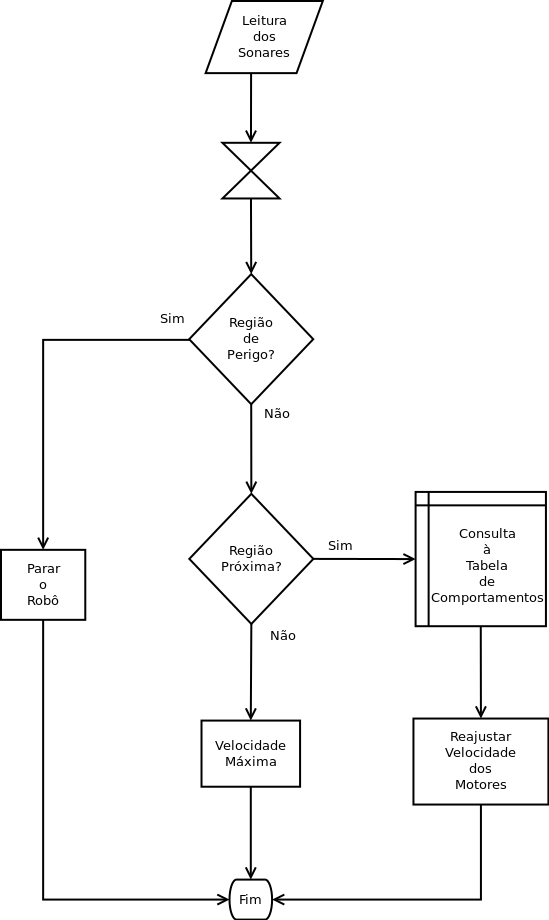
\includegraphics[width=0.8 \linewidth]{../../Imagens/ObstAvoid.png}
    \caption{Fluxograma da Rotina de Desvio de Obstáculos}
    \label{ObstAvoid}
  \end{figure}

\section{Sistemas de Tempo Real}
São sistemas computacionais que dependem não somente que os dados computados estejam corretos, mas que sejam obtidos dentro de um intervalo de tempo 
pré determinado, que pode ser maior ou menor de acordo com a aplicação.
Na literatura, este período em que se espera que a resposta do sistema se dê é denominado \textit{deadline}.
Sistemas de tempo real podem ser classificados em dois tipos: \textit{soft} ou \textit{hard}.

Sistemas \textit{soft} são menos restritivos, tolerando eventuais perdas de \textit{deadline}; 
ao contrário dos sistemas \textit{hard}, em que estas perdas não são aceitáveis.  

Algumas características típicas, apesar de não obrigatórias, de sistemas de tempo real são limitações com relação ao tamanho, propósito específico e 
baixo custo \cite{silberschatz}.

\section{CRC}
Método de detecção de erros aleatórios, isto é, de dados corrompidos ao longo do processo de transmissão ou armazenamento da informação por exemplo 
por ruídos, mas não por um agente \textquoteleft inteligente\textquoteright{} externo que modifique os dados transmitidos, tal qual um 
\textit{malware} \cite{stigge}.

Consiste essencialmente em uma divisão polinomial \cite{stigge}, logo, pode ser implementado em \textit{hardware}, utilizando-se apenas registradores 
de deslocamento com conexões realimentadas \cite{peterson}, assim como em \textit{software}. 
Em suma, trata-se de acrescentar à mensagem digital original um sufixo, que tem seu valor definido por operações realizadas em função da mensagem 
binária que intenta-se enviar e de um polinômio gerador.
Para o \textit{transceiver} nRF24L01+, dois polinômios geradores são utilizados: Eq. \ref{CRC_1} quando o dado cíclico adicionado é de 1 
\textit{byte} , e Eq. \ref{CRC_2}, para 2 \textit{bytes} \cite{nRF}.

Para uma descrição completa de como é implementado este método, vide \cite{stigge,peterson}.

\begin{equation}
\label{CRC_1}
G(X) = X^8 + X^2 + X + 1 
\end{equation}

\begin{equation}
\label{CRC_2}
G(X) = X^{16} + X^{12} + X^5 + 1 
\end{equation}

\section{MIFA} %% se der tempo, né?

\section{efeito hall} %% se der tempo, né?

\section{campo girante}

\section{\textit{schmitt trigger}}

\section{PWM}
A modulação por largura de pulso é uma técnica de modulação que consiste em amostrar e codificar o sinal correspondente à mensagem na largura de um 
trem de pulsos de amplitude fixa, i.e. cada amostra da mensagem é convertida em um pulso retangular cuja duração expressa a amplitude do sinal 
modulante.

Um modulador PWM pode ser implementado utilizando-se um circuito comparador não inversor cuja entrada inversora liga-se à saída de um gerador de 
ondas tipo dente de serra (\textit{trailing edge modulation}), dente de serra invertida (\textit{leading edge modulation}  ou triangular 
(\textit{modulation on both edges}), na entrada não inversora, o sinal modulante. 
Desta forma, quando a tensão da mensagem excede a amplitude da onda gerada, observa-se um sinal alto na saída, caso contrário, baixo, conforme 
ilustra a Fig. \ref{pwm_modulation_types}.

  \begin{figure}[!htb] %% TODO fonte: https://en.wikipedia.org/wiki/File:Three_PWM_types.svg
    \centering
    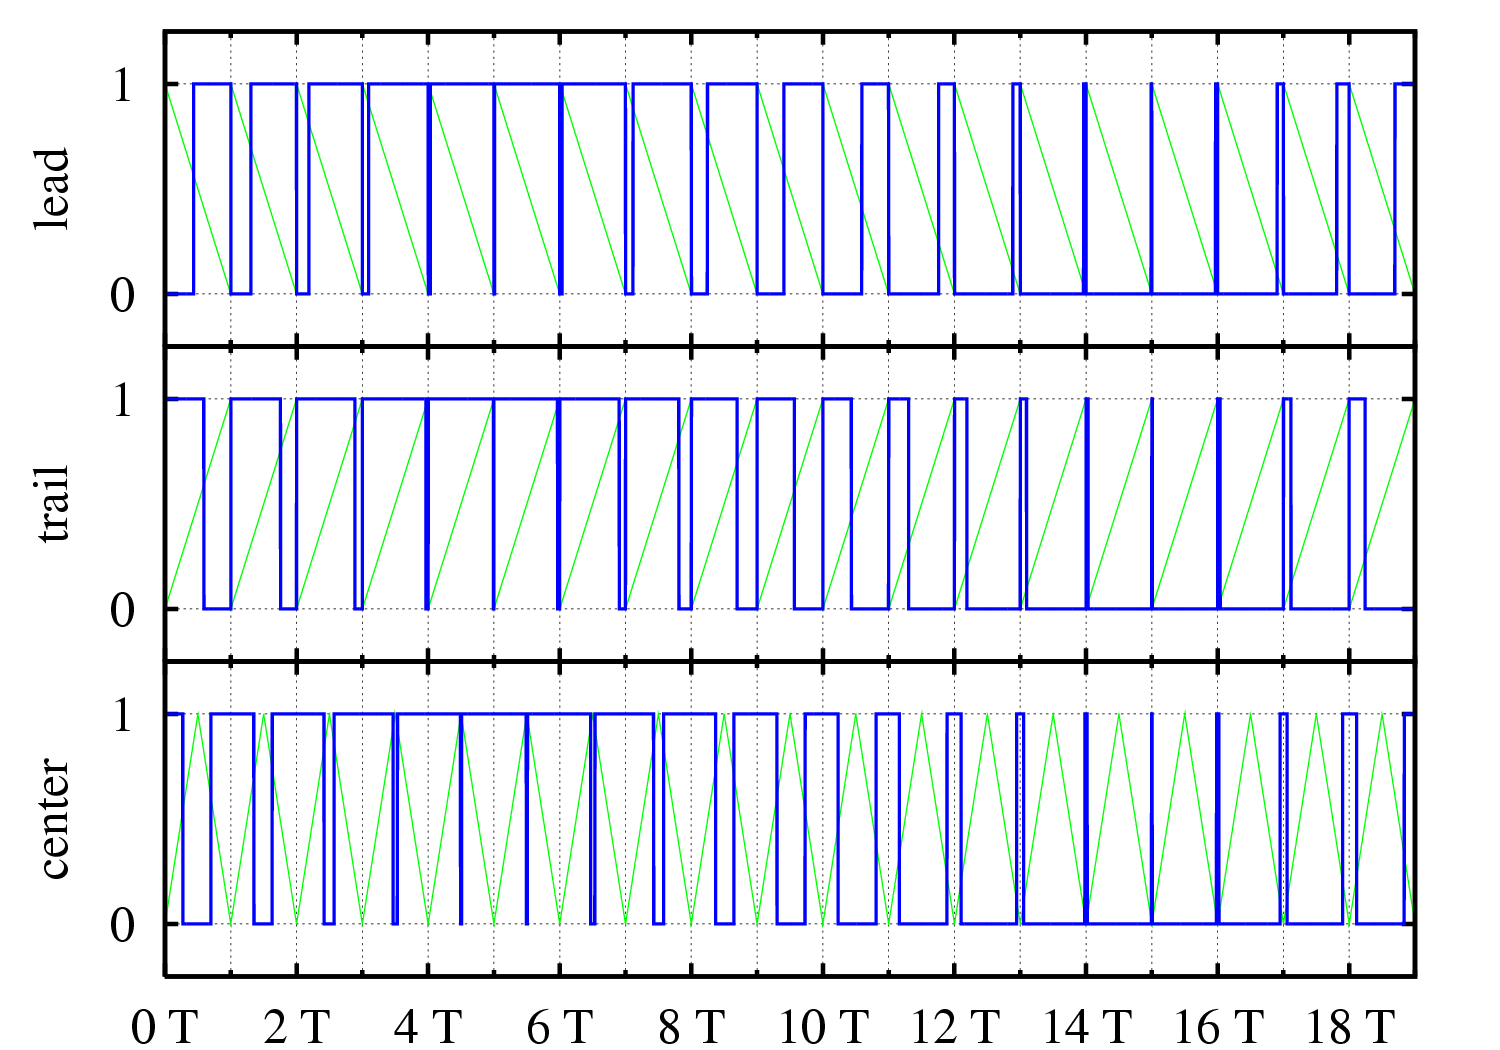
\includegraphics[width=0.7\linewidth]{../../Imagens/PWM_modulation_types.png}
    \caption{Três tipos de modulação PWM: \textit{trailing edge}, \textit{leading edge} e  \textit{both edges}, de cima pra baixo, respectivamente.}
    \label{pwm_modulation_types}
  \end{figure}
  
  %TODO circuito corretor de erros:
   First, the error amplifier accommodates feedback of the output PWM waveform in order to correct for any errors in the
output voltage introduced by the comparator. Second, it adds a dc offset to the input voltage so that negative input voltages can be accommodated by 
the circuit.
 
 Because the supply voltage of the comparator directly impacts the output voltage, PWM circuits without feedback have no power supply rejection. In 
this TI Design, the error amplifier acts as an inverting amplifier to the input signal, shown as a dc-coupled source VIN. By including the comparator 
inside the feedback loop of the error amplifier, and adding integration capacitor C1, the error amplifier now directly controls the average output 
voltage



para uma descrição detalhada do circuito e simulações vide \cite{pwm_modulator}

\section{GFSK}

\section{banda ISM}

\section{SPI}

\section{Testes Realizados}
\subsection{Interferência dos BLDC nos sonares}
\begin{table}[]
\centering
\caption{My caption}
\label{my-label}
\begin{tabular}{lllll|l|}
\hline
\multicolumn{1}{|c|}{\textbf{USS4}} & \multicolumn{1}{c|}{\textbf{USS3}} & \multicolumn{1}{c|}{\textbf{USS2}} & \multicolumn{1}{c|}{\textbf{USS1}} & 
\multicolumn{1}{c|}{\textbf{USS0}} & \multicolumn{1}{c|}{\textbf{Manobra}} \\ \hline
\multicolumn{1}{c}{273}             & \multicolumn{1}{c}{400}            & \multicolumn{1}{c}{400}            & \multicolumn{1}{c}{82}             & 
400                                & DF                                    \\ \hline
\multicolumn{1}{c}{211}             & \multicolumn{1}{c}{400}            & \multicolumn{1}{c}{400}            & \multicolumn{1}{c}{188}            & 
400                                & DF                                    \\ \hline
161                                 & 400                                & 400                                & 294                                & 
400                                & DF                                    \\ \hline
112                                 & 400                                & 400                                & 400                                & 
400                                & DF                                    \\ \hline
111                                 & 400                                & 400                                & 400                                & 
400                                & DF                                    \\ \hline
112                                 & 400                                & 400                                & 400                                & 
400                                & DF                                    \\ \hline
113                                 & 400                                & 400                                & 400                                & 
400                                & DF                                    \\ \hline
112                                 & 400                                & 400                                & 400                                & 
400                                & DF                                    \\ \hline
111                                 & 400                                & 400                                & 400                                & 
400                                & DF                                    \\ \hline
112                                 & 400                                & 400                                & 400                                & 
400                                & DF                                    \\ \hline
111                                 & 400                                & 400                                & 400                                & 
400                                & DF                                    \\ \hline
112                                 & 400                                & 400                                & 400                                & 
400                                & DF                                    \\ \hline
111                                 & 400                                & 400                                & 400                                & 
400                                & DF                                    \\ \hline
112                                 & 400                                & 400                                & 400                                & 
400                                & DF                                    \\ \hline
113                                 & 400                                & 400                                & 400                                & 
400                                & DF                                    \\ \hline
112                                 & 400                                & 400                                & 400                                & 
400                                & DF                                    \\ \hline
113                                 & 400                                & 400                                & 400                                & 
400                                & DF                                    \\ \hline
112                                 & 400                                & 400                                & 400                                & 
400                                & DF                                    \\ \hline
113                                 & 400                                & 400                                & 400                                & 
400                                & DF                                    \\ \hline
112                                 & 400                                & 400                                & 400                                & 
400                                & DF                                    \\ \hline
111                                 & 400                                & 400                                & 400                                & 
400                                & DF                                    \\ \hline
110                                 & 400                                & 400                                & 400                                & 
400                                & DF                                    \\ \hline
111                                 & 400                                & 400                                & 400                                & 
400                                & DF                                    \\ \hline
112                                 & 400                                & 400                                & 400                                & 
400                                & DF                                    \\ \hline
113                                 & 400                                & 400                                & 400                                & 
400                                & DF                                    \\ \hline
113                                 & 400                                & 400                                & 400                                & 
303                                & FS                                    \\ \hline
113                                 & 400                                & 400                                & 400                                & 
205                                & FS                                    \\ \hline
208                                 & 400                                & 400                                & 400                                & 
205                                & FS                                    \\ \hline
304                                 & 400                                & 400                                & 400                                & 
302                                & FS                                    \\ \hline
400                                 & 400                                & 400                                & 400                                & 
303                                & EF                                    \\ \hline
400                                 & 400                                & 400                                & 400                                & 
207                                & EF                                    \\ \hline
400                                 & 400                                & 400                                & 400                                & 
110                                & EF                                    \\ \hline
400                                 & 400                                & 400                                & 400                                & 
109                                & EF                                    \\ \hline
400                                 & 400                                & 400                                & 400                                & 
207                                & EF                                    \\ \hline
400                                 & 400                                & 400                                & 400                                & 
208                                & EF                                    \\ \hline
400                                 & 400                                & 400                                & 400                                & 
304                                & EF                                    \\ \hline
400                                 & 400                                & 400                                & 400                                & 
400                                & OR                                    \\ \hline
400                                 & 400                                & 400                                & 400                                & 
304                                & EF                                    \\ \hline
400                                 & 400                                & 400                                & 400                                & 
209                                & EF                                    \\ \hline
400                                 & 400                                & 400                                & 400                                & 
114                                & EF                                    \\ \hline
400                                 & 400                                & 400                                & 400                                & 
113                                & EF                                    \\ \hline
400                                 & 400                                & 400                                & 400                                & 
114                                & EF                                    \\ \hline
400                                 & 400                                & 400                                & 400                                & 
113                                & EF                                    \\ \hline
400                                 & 400                                & 400                                & 400                                & 
114                                & EF                                    \\ \hline
400                                 & 400                                & 400                                & 400                                & 
115                                & EF                                    \\ \hline
400                                 & 400                                & 400                                & 400                                & 
114                                & EF                                    \\ \hline
400                                 & 400                                & 400                                & 400                                & 
115                                & EF                                    \\ \hline
400                                 & 400                                & 400                                & 400                                & 
114                                & EF                                    \\ \hline
400                                 & 400                                & 400                                & 400                                & 
115                                & EF                                    \\ \hline
400                                 & 400                                & 400                                & 400                                & 
114                                & EF                                    \\ \hline
400                                 & 400                                & 400                                & 400                                & 
115                                & EF                                    \\ \hline
400                                 & 400                                & 400                                & 400                                & 
116                                & EF                                    \\ \hline
400                                 & 400                                & 400                                & 400                                & 
211                                & EF                                    \\ \hline
400                                 & 400                                & 400                                & 400                                & 
305                                & EF                                    \\ \hline
400                                 & 400                                & 400                                & 400                                & 
400                                & OR                                    \\ \hline
301                                 & 400                                & 400                                & 400                                & 
400                                & DF                                    \\ \hline
201                                 & 400                                & 400                                & 400                                & 
400                                & DF                                    \\ \hline
100                                 & 400                                & 400                                & 400                                & 
400                                & DF                                    \\ \hline
98                                  & 400                                & 400                                & 400                                & 
400                                & DF                                    \\ \hline
96                                  & 400                                & 400                                & 400                                & 
400                                & DF                                    \\ \hline
95                                  & 400                                & 400                                & 400                                & 
400                                & DF                                    \\ \hline
94                                  & 400                                & 400                                & 400                                & 
400                                & DF                                    \\ \hline
93                                  & 400                                & 400                                & 400                                & 
400                                & DF                                    \\ \hline
94                                  & 400                                & 400                                & 400                                & 
400                                & DF                                    \\ \hline
95                                  & 400                                & 400                                & 400                                & 
400                                & DF                                    \\ \hline
94                                  & 400                                & 400                                & 400                                & 
400                                & DF                                    \\ \hline
93                                  & 400                                & 400                                & 400                                & 
400                                & DF                                    \\ \hline
94                                  & 400                                & 400                                & 400                                & 
400                                & DF                                    \\ \hline
93                                  & 400                                & 400                                & 400                                & 
400                                & DF                                    \\ \hline
94                                  & 400                                & 400                                & 400                                & 
400                                & DF                                    \\ \hline
95                                  & 400                                & 400                                & 400                                & 
400                                & DF                                    \\ \hline
94                                  & 400                                & 400                                & 400                                & 
400                                & DF                                    \\ \hline
95                                  & 400                                & 400                                & 400                                & 
400                                & DF                                    \\ \hline
94                                  & 400                                & 400                                & 400                                & 
400                                & DF                                    \\ \hline
95                                  & 400                                & 400                                & 400                                & 
400                                & DF                                    \\ \hline
94                                  & 400                                & 400                                & 400                                & 
400                                & DF                                    \\ \hline
93                                  & 400                                & 400                                & 400                                & 
400                                & DF                                    \\ \hline
94                                  & 400                                & 400                                & 400                                & 
400                                & DF                                    \\ \hline
95                                  & 400                                & 400                                & 400                                & 
400                                & DF                                    \\ \hline
96                                  & 400                                & 400                                & 400                                & 
400                                & DF                                    \\ \hline
97                                  & 400                                & 400                                & 400                                & 
400                                & DF                                    \\ \hline
99                                  & 400                                & 400                                & 400                                & 
400                                & DF                                    \\ \hline
100                                 & 400                                & 400                                & 400                                & 
400                                & DF                                    \\ \hline
103                                 & 400                                & 400                                & 400                                & 
400                                & DF                                    \\ \hline
202                                 & 400                                & 400                                & 400                                & 
400                                & DF                                    \\ \hline
302                                 & 400                                & 400                                & 400                                & 
400                                & DF                                    \\ \hline
400                                 & 400                                & 400                                & 400                                & 
400                                & OR                                    \\ \hline
400                                 & 400                                & 400                                & 400                                & 
303                                & EF                                    \\ \hline
400                                 & 400                                & 400                                & 400                                & 
206                                & EF                                    \\ \hline
400                                 & 400                                & 400                                & 400                                & 
108                                & EF                                    \\ \hline
400                                 & 400                                & 400                                & 400                                & 
106                                & EF                                    \\ \hline
400                                 & 400                                & 400                                & 400                                & 
105                                & EF                                    \\ \hline
400                                 & 400                                & 400                                & 400                                & 
104                                & EF                                    \\ \hline
400                                 & 400                                & 400                                & 365                                & 
104                                & EF                                    \\ \hline
400                                 & 400                                & 400                                & 267                                & 
103                                & EF                                    \\ \hline
400                                 & 400                                & 400                                & 267                                & 
101                                & EF                                    \\ \hline
400                                 & 400                                & 400                                & 169                                & 
100                                & EF                                    \\ \hline
400                                 & 400                                & 400                                & 106                                & 
99                                 & EF                                    \\ \hline
400                                 & 400                                & 400                                & 105                                & 
99                                 & EF                                    \\ \hline
400                                 & 400                                & 400                                & 105                                & 
100                                & EF                                    \\ \hline
400                                 & 400                                & 400                                & 105                                & 
101                                & EF                                    \\ \hline
400                                 & 400                                & 400                                & 105                                & 
100                                & EF                                    \\ \hline
400                                 & 400                                & 400                                & 105                                & 
99                                 & EF                                    \\ \hline
400                                 & 400                                & 400                                & 105                                & 
98                                 & EF                                    \\ \hline
400                                 & 400                                & 400                                & 104                                & 
97                                 & EF                                    \\ \hline
400                                 & 400                                & 400                                & 104                                & 
80                                 & EF                                    \\ \hline
400                                 & 400                                & 400                                & 104                                & 
64                                 & EF                                    \\ \hline
400                                 & 400                                & 400                                & 104                                & 
48                                 & STP                                   \\ \hline
400                                 & 400                                & 400                                & 104                                & 
49                                 & STP                                   \\ \hline
400                                 & 400                                & 400                                & 105                                & 
49                                 & STP                                   \\ \hline
400                                 & 400                                & 400                                & 104                                & 
49                                 & STP                                   \\ \hline
400                                 & 400                                & 400                                & 105                                & 
49                                 & STP                                   \\ \hline
400                                 & 400                                & 400                                & 105                                & 
65                                 & EF                                    \\ \hline
400                                 & 400                                & 400                                & 105                                & 
82                                 & EF                                    \\ \hline
400                                 & 400                                & 400                                & 105                                & 
97                                 & EF                                    \\ \hline
400                                 & 400                                & 400                                & 105                                & 
98                                 & EF                                    \\ \hline
400                                 & 400                                & 400                                & 106                                & 
98                                 & EF                                    \\ \hline
400                                 & 400                                & 400                                & 204                                & 
100                                & EF                                    \\ \hline
400                                 & 400                                & 400                                & 302                                & 
102                                & EF                                    \\ \hline
400                                 & 400                                & 400                                & 400                                & 
105                                & EF                                    \\ \hline
400                                 & 400                                & 400                                & 400                                & 
108                                & EF                                    \\ \hline
400                                 & 400                                & 400                                & 400                                & 
110                                & EF                                    \\ \hline
400                                 & 400                                & 400                                & 400                                & 
112                                & EF                                    \\ \hline
400                                 & 400                                & 400                                & 400                                & 
114                                & EF                                    \\ \hline
400                                 & 400                                & 400                                & 400                                & 
115                                & EF                                    \\ \hline
400                                 & 400                                & 400                                & 400                                & 
114                                & EF                                    \\ \hline
400                                 & 400                                & 400                                & 400                                & 
113                                & EF                                    \\ \hline
400                                 & 400                                & 400                                & 400                                & 
112                                & EF                                    \\ \hline
400                                 & 400                                & 400                                & 400                                & 
113                                & EF                                    \\ \hline
400                                 & 400                                & 400                                & 400                                & 
210                                & EF                                    \\ \hline
400                                 & 400                                & 400                                & 400                                & 
305                                & EF                                    \\ \hline
400                                 & 400                                & 400                                & 400                                & 
400                                & OR                                    \\ \hline
303                                 & 400                                & 400                                & 400                                & 
400                                & DF                                    \\ \hline
205                                 & 400                                & 400                                & 400                                & 
400                                & DF                                    \\ \hline
303                                 & 400                                & 400                                & 400                                & 
400                                & DF                                    \\ \hline
400                                 & 400                                & 400                                & 400                                & 
400                                & OR                                    \\ \hline
302                                 & 400                                & 400                                & 400                                & 
400                                & DF                                    \\ \hline
203                                 & 400                                & 400                                & 400                                & 
400                                & DF                                    \\ \hline
104                                 & 400                                & 400                                & 400                                & 
400                                & DF                                    \\ \hline
103                                 & 400                                & 400                                & 400                                & 
400                                & DF                                    \\ \hline
85                                  & 400                                & 400                                & 400                                & 
400                                & DF                                    \\ \hline
66                                  & 400                                & 400                                & 400                                & 
400                                & DF                                    \\ \hline
47                                  & 400                                & 400                                & 400                                & 
400                                & STP                                   \\ \hline
39                                  & 400                                & 400                                & 400                                & 
400                                & STP                                   \\ \hline
49                                  & 400                                & 400                                & 400                                & 
400                                & STP                                   \\ \hline
31                                  & 400                                & 400                                & 400                                & 
400                                & STP                                   \\ \hline
42                                  & 400                                & 400                                & 400                                & 
400                                & STP                                   \\ \hline
58                                  & 400                                & 400                                & 400                                & 
400                                & DF                                    \\ \hline
73                                  & 400                                & 400                                & 400                                & 
400                                & DF                                    \\ \hline
74                                  & 400                                & 400                                & 400                                & 
400                                & DF                                    \\ \hline
75                                  & 400                                & 400                                & 400                                & 
400                                & DF                                    \\ \hline
81                                  & 400                                & 400                                & 400                                & 
400                                & DF                                    \\ \hline
86                                  & 400                                & 400                                & 400                                & 
400                                & DF                                    \\ \hline
90                                  & 400                                & 400                                & 400                                & 
400                                & DF                                    \\ \hline
90                                  & 400                                & 400                                & 278                                & 
400                                & DF                                    \\ \hline
90                                  & 400                                & 400                                & 156                                & 
400                                & DF                                    \\ \hline
93                                  & 400                                & 400                                & 39                                 & 
400                                & DF                                    \\ \hline
94                                  & 400                                & 400                                & 37                                 & 
400                                & DF                                    \\ \hline
97                                  & 400                                & 400                                & 43                                 & 
400                                & DF                                    \\ \hline
100                                 & 400                                & 400                                & 49                                 & 
400                                & DF                                    \\ \hline
101                                 & 400                                & 400                                & 51                                 & 
400                                & DF                                    \\ \hline
101                                 & 400                                & 400                                & 56                                 & 
400                                & DF                                    \\ \hline
101                                 & 400                                & 400                                & 60                                 & 
400                                & DF                                    \\ \hline
105                                 & 400                                & 400                                & 63                                 & 
400                                & DF                                    \\ \hline
108                                 & 400                                & 400                                & 70                                 & 
400                                & DF                                    \\ \hline
193                                 & 400                                & 400                                & 74                                 & 
400                                & DF                                    \\ \hline
290                                 & 400                                & 400                                & 74                                 & 
400                                & DF                                    \\ \hline
385                                 & 400                                & 400                                & 78                                 & 
400                                & OR                                    \\ \hline
400                                 & 400                                & 400                                & 79                                 & 
400                                & OR                                    \\ \hline
393                                 & 400                                & 400                                & 80                                 & 
400                                & OR                                    \\ \hline
387                                 & 400                                & 400                                & 81                                 & 
400                                & OR                                    \\ \hline
379                                 & 400                                & 400                                & 82                                 & 
400                                & OR                                    \\ \hline
377                                 & 400                                & 400                                & 83                                 & 
400                                & OR                                    \\ \hline
374                                 & 400                                & 400                                & 84                                 & 
400                                & OR                                    \\ \hline
                                    &                                    &                                    &                                    &   
                                 &                                       \\ \hline
\end{tabular}
\end{table}